\documentclass[a4paper]{article}
\usepackage{graphicx,placeins}
\usepackage{epsfig}
\usepackage{comment}
\usepackage{amsmath,amsthm}
\usepackage{xspace}
\usepackage[colorlinks=true,citecolor=blue]{hyperref}
\usepackage[acronym,nonumberlist,nogroupskip]{glossaries}
\usepackage{showlabels}

\newcommand{\etal}{{\it et~al.}\ }
\newcommand{\ie}{{\it i.e.}\ }
\newcommand{\eg}{{\it e.g.}\ }
\newcommand{\Ito}{It\^{o} }
\newcommand{\tsing}{t_{\text{singular}}}
\newcommand{\gest}{g_{\text{est}}}
\newcommand{\eq}{\hspace{-.15cm}=\hspace{-.15cm}}
\newcommand{\ave}[1]{\left\langle#1 \right\rangle}
\newcommand{\dist}{\,{\buildrel d \over =}\,}
\newcommand{\mut}{\tilde{\mu}}
\newcommand{\sigmat}{\tilde{\sigma}}
\newcommand{\var}{\text{var}}
\newcommand{\PDF}{\mathcal{P}}

\newcommand{\rex}{r_{\ave{}}}
\newcommand{\rt}{r_{t}}

\newcommand{\gt}{g_{t}}


\newcommand{\elabel}[1]{\label{eq:#1}}
\newcommand{\eref}[1]{(Eq.~\ref{eq:#1})}
\newcommand{\Eref}[1]{Equation~(\ref{eq:#1})}

\newcommand{\ceref}[2]{(\ref{eq:#1}#2)}

\newcommand{\tlabel}[1]{\label{tab:#1}}
\newcommand{\tref}[1]{(Table~\ref{tab:#1})}

\newcommand{\flabel}[1]{\label{fig:#1}}
\newcommand{\fref}[1]{Fig.~\ref{fig:#1}}
\newcommand{\Fref}[1]{Figure ~\ref{fig:#1}}

\newcommand{\seclabel}[1]{\label{section:#1}}
\newcommand{\secref}[1]{Sec.~\ref{section:#1}}
\newcommand{\Secref}[1]{Section~\ref{section:#1}}

\newcommand{\OP}[1]{{\bf @@@OP: #1 @@@}}
\renewcommand{\AA}[1]{{\bf ===AA: #1 ===}}

\newcommand{\be}{\begin{equation}}
\newcommand{\ee}{\end{equation}}
\newcommand{\bea}{\begin{eqnarray}}
\newcommand{\eea}{\end{eqnarray}}
\newcommand{\bc}{\begin{center}}
\newcommand{\ec}{\end{center}}
\newcommand{\prob}[1]{\mathcal{P}\left(#1\right)}
\newcommand{\D}{\Delta}
\newcommand{\nn}{\nonumber}

\newcommand{\definition}[1]{\vspace{.2cm} {\bf \underline{Definition} #1} \vspace{.2cm}}


\begin{document}

\title{Ergodicity Economics}
\author{Ole Peters and Alexander Adamou\\
London Mathematical Laboratory\\
14 Buckingham Street, London WC2N 6DF, UK}
\date{\today}
\maketitle
\begin{abstract}

\end{abstract}

\tableofcontents
\newpage

\section{Tossing a coin}
\subsection{The game}
\seclabel{The_game}
Imagine I offer you the following game: I toss a coin, and if it comes 
up heads I increase your monetary wealth by 50\%; if 
it comes up tails I reduce your wealth by 40\%. I'm not only 
doing this once, I will do it many times, for example 
once per week for the rest of your life. Would you accept 
the rules of my game? Would you submit your wealth to 
the dynamic my game will impose on it?

Your answer to this question is up to you and will be 
influenced by many factors, such as the importance 
you attach to wealth that can be measured in monetary 
terms, whether you like the thrill of gambling, your 
religion and moral convictions and so on.

In these notes we will mostly ignore these aspects.
We will build an extremely simple model of your 
wealth, which will lead to an extremely simple
powerful model of the way you make decisions that affect 
your wealth. We are interested in analyzing the 
game mathematically, which requires a translation 
of the game into mathematics. We choose the 
following translation: we introduce the key 
variable, $x(t)$, which we refer to as ``wealth''. 
We refer to $t$ as ``time''. It should be kept in mind that
``wealth'' and ``time'' are just names that we've given to 
mathematical objects. We have chosen these names because
we want to compare the behaviour of the mathematical
objects to the behaviour of wealth over time, but
we emphasize that we're building a model -- whether we write $x(t)$ 
or $\text{wealth}(\text{time})$ makes no difference to the mathematics. 
The usefulness of our model will be different in different circumstances, 
ranging from completely meaningless to very helpful. There is no 
substitute for careful consideration of any given situation, and
labeling mathematical objects in one way or another is certainly none.

Having got these words of warning out of the way, we define our 
model of the dynamics of your wealth under the rules we specified. 
In each time step of duration $\D t$ we randomly generate a 
factor $r(t)$ with each of possible values
$r_i\in \{0.6, 1.5\}$ occurring with probability 1/2, 

\be 
r(t) = \begin{cases}
0.6 &\text{with probability  1/2}\\
1.5 &\text{with probability 1/2}
\end{cases}
\elabel{law}
\ee
and multiply current wealth by that factor, 
\be
x(t+\Delta t)=r(t)\times x(t).
\elabel{gamble}
\ee


Without discussing in depth how realistic a representation of your 
wealth this model is (for instance your non-gambling related 
income and spending are not represented in the model),
 and without discussing whether randomness truly exists and 
what the meaning of a probability is we simply switch on a 
computer and simulate what might happen. You may have many 
good ideas of how to analyze our game with pen and paper, 
but we will just generate possible trajectories of your wealth 
and pretend we know nothing about mathematics or 
economic theory. \Fref{1_1} is a trajectory of your wealth, 
according to our computer model as it might evolve over 
the course of 52 time steps (corresponding to one year given our 
original setup).

\begin{figure}[h!]
\begin{picture}(200,160)(0,0)
    \put(0,-85){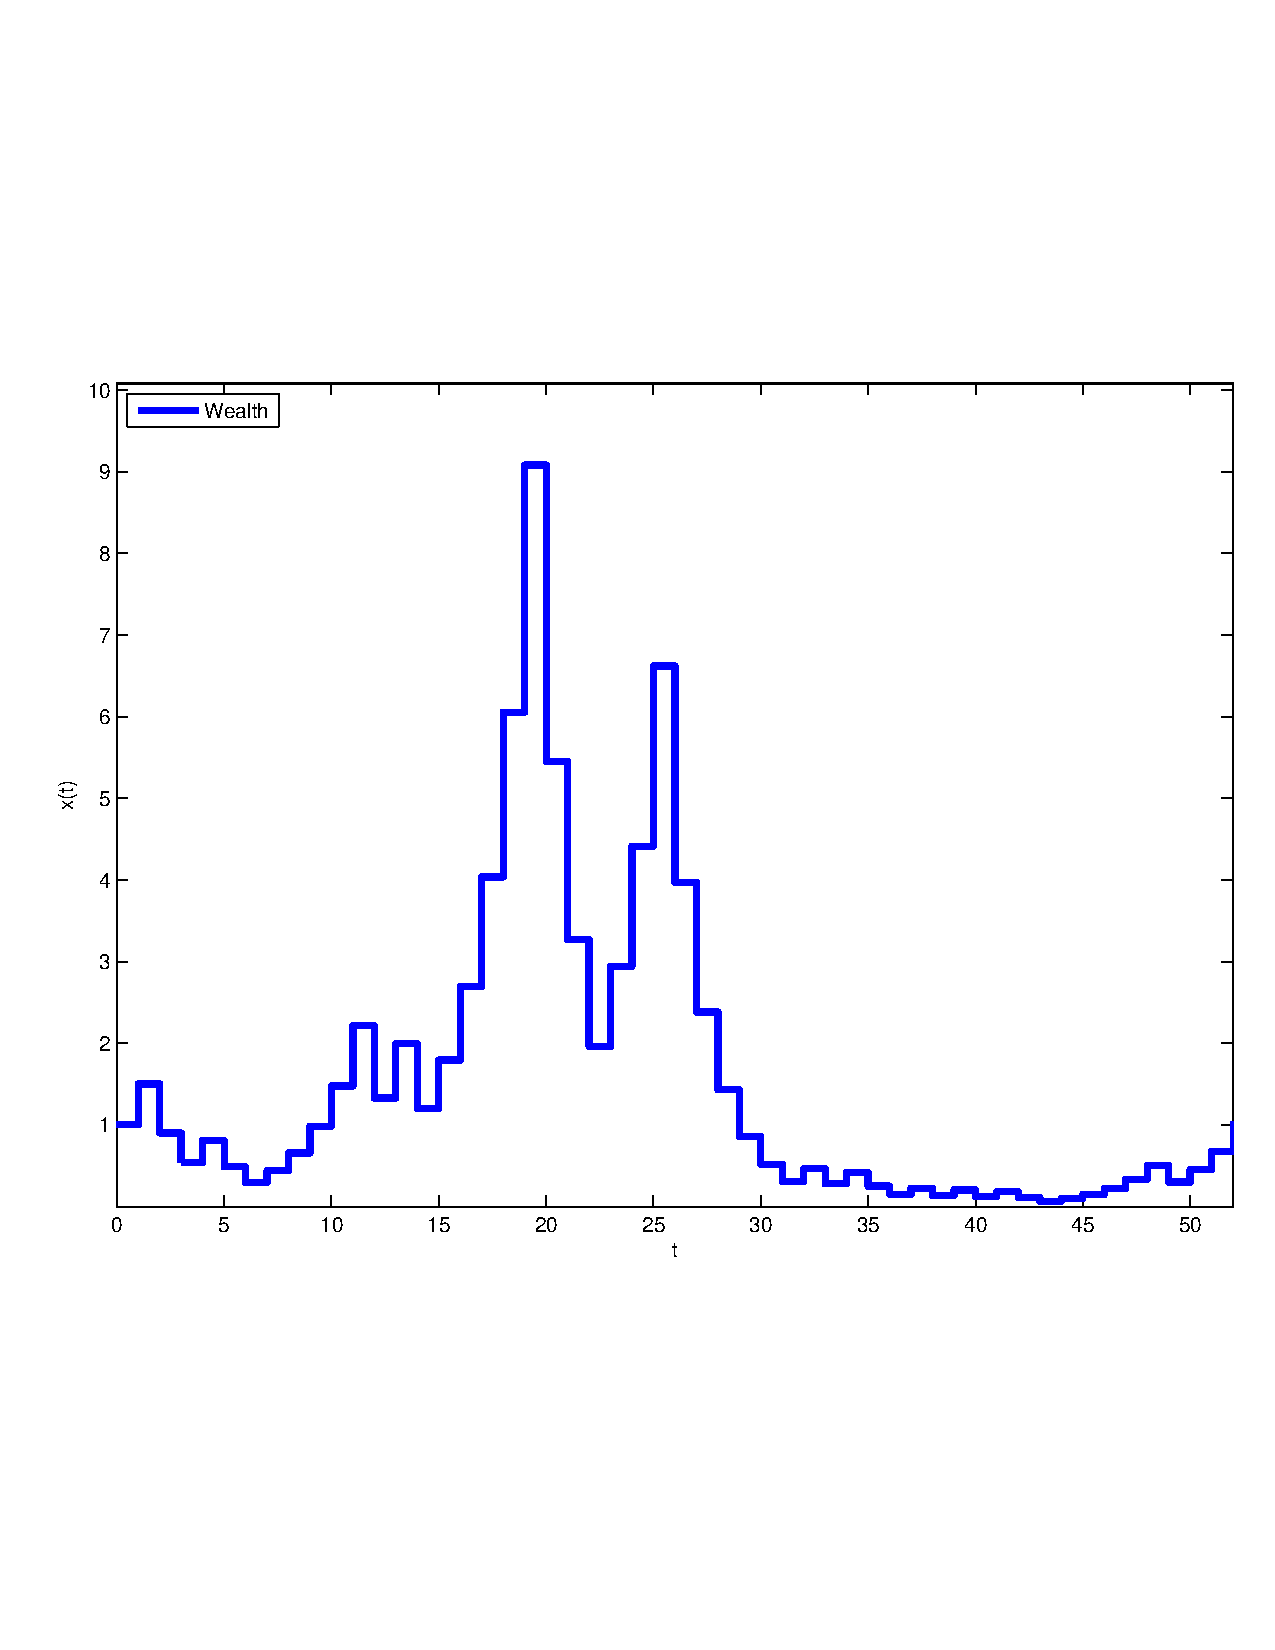
\includegraphics[width=0.8\textwidth]{./figs/fig1_1.pdf}}
\end{picture}
\caption{Wealth $x(t)$ resulting from a computer simulation of our game, repeated 52 times.}
\flabel{1_1}
\end{figure}


A cursory glance at the trajectory does not reveal much structure. 
Of course there are regularities, for instance at each time step 
$x(t)$ changes, but no trend is discernible -- does this trajectory 
have a tendency to go up, does it have a tendency to go down? 
Neither? What are we to learn from this simulation? Perhaps we 
conclude that playing the game for a year is quite risky, but is the 
risk worth taking? 

An early invention in the development of probability theory is the 
expectation value. This invention was made in the 
context of gambling, and we're investigating a game that seems like a 
gamble. So it may be useful to us. We denote the expectation
value of $x$ by placing angled brackets around $x$, like this: $\ave{x}$. 
Sometimes this is called Dirac notation. The expectation value 
is usually introduced as a weighted sum.

\definition{The expectation value of a quantity $x$ 
that can take discrete values $x_j$ is the sum of all 
possible values weighted by their probabilities $p_j$
\be
\ave{x}=\sum_k p_j x_j.
\ee 
If $x$ is continuous, the expectation value is the integral
\be
\ave{x}=\int_{-\infty}^{+\infty} ds \PDF_x(s) ds,
\ee where $\PDF_x(s)$ is the probability density function (PDF)
of the random variable $x$ at value $s$. Another word for ``expectation value'' is
``ensemble average.''}

Computationally, we can find the expectation value of $x$ at some
specific time $t^*$ as follows:
\begin{itemize}
\item
generate an ensemble of $N$ trajectories 
$x_i(t)$ according to \eref{gamble}
\item
collect the $N$ values $x_i(t^*)$ at the time of interest
\item
compute the finite-ensemble average 
$\ave{x}_N=\frac{1}{N}\sum_i x_i(t^*)$.
\end{itemize}
In the large-ensemble limit $N\to\infty$, the finite-ensemble average 
$\ave{x}_N$ converges to the expectation value $\ave{x}$ with probability 1.
If this is unclear, consider the number of times
the value $x_j$ is observed at time $t$. Call this $n_j$. 
The finite-ensemble average can then be re-written as
\bea
\ave{x}_N&=&\frac{1}{N}\sum_i  x_i(t^*)\\
&=&\sum_j \frac{n_j}{N} x_j(t^*).
\eea
The fraction $\frac{n_j}{N}$ in the limit $N\to\infty$ may be
considered the definition of the probability $p_j$, and we find
\bea
\lim_{N\to\infty}\ave{x(t^*)}_N&=&\sum_j p_j x_j(t^*)\\
&=&\ave{x(t^*)}.
\eea

%To compute the 
%expectation value of some quantity $A$ we need the following:
%\begin{itemize}
%\item
%a list of all possible future states of the universe, $i$
%\item
%the quantity $A_i$ in each imagined universe
%\item
%probability $p_i$ of each imagined universe
%\end{itemize}
%Of course the items in this list constitute a model. A possible
%future state of the universe cannot be observed, it's not physical (yet), 
%but just a hypothetical state of affairs. Similarly, the value of $A$ in
%some hypothetical state is hypothetical and unobservable, as is 
%indeed the probability of some hypothetical state. In other words, for
%the expectation value of some real observable quantity 
%to be computed, we need to invent a model of how that quantity
%behaves in different universes and how likely those universes are.
%
%Luckily, we've already completed this very difficult step. We have decided
%to model wealth as behaving according to \eref{law}, and this allows us
%to compute the expectation value.

The exact probability of reaching wealth $x_j(t^*)$ at time $t^*$ is 
the number of all distinct trajectories that turn the stating wealth into $x_j(t^*)$, divided by the 
number of all possible distinct trajectories up to that time $t^*$. At time $t^*=52$ the 
number of all distinct trajectories is $2^{52}=4,503,599,627,370,496$ so attmpting to 
count exactly will get us into trouble. But computational physics has provided us with the 
powerful tool of Monte Carlo simulation. Instead of actually counting all possibilities we 
can just generate a large number of equally likely random trajectories and average 
over them. As the number of trajectories in our average increases, the result
will converge to the expectation value,
\be
\ave{x(t)}=\lim_{N\to\infty} \frac{1}{N}\sum_i^N x_i(t).
\elabel{ave_x}
\ee
The collection of all possible trajectories $\{x_i(t)\}$ is called 
an ensemble, and because the expectation value can be 
obtained by averaging over all ensemble members it is also 
called the ensemble average. In \fref{1_2} we approximate 
the expectation value in a Monte Carlo simulation. By 
successively adding random trajectories to a finite ensemble, 
the randomness in the finite-ensemble average is 
systematically removed.
\begin{figure}[h!]
\begin{picture}(200,250)(0,0)
  \put(-50,30){(A)}
    \put(-100,-30){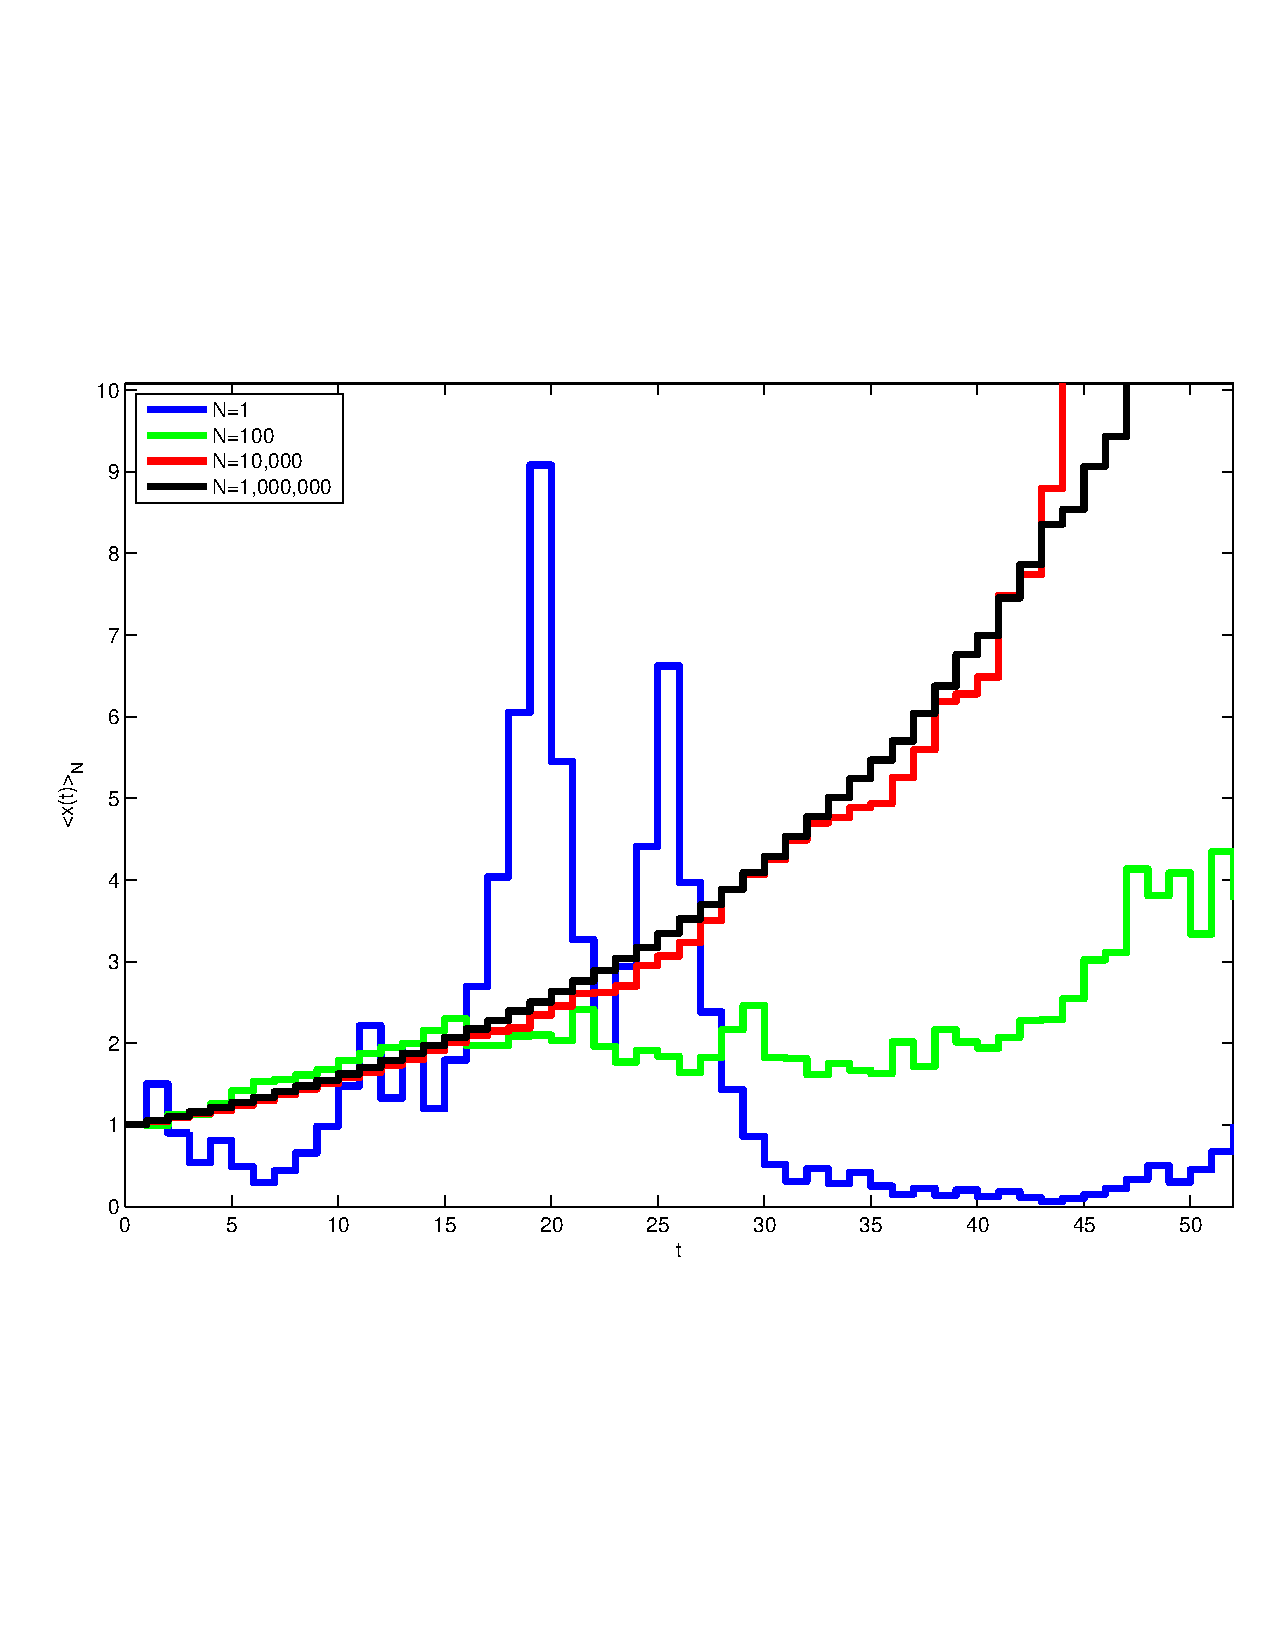
\includegraphics[width=0.8\textwidth]{./figs/fig1_2a.pdf}}
  \put(230,30){(B)}  
  \put(180,-30){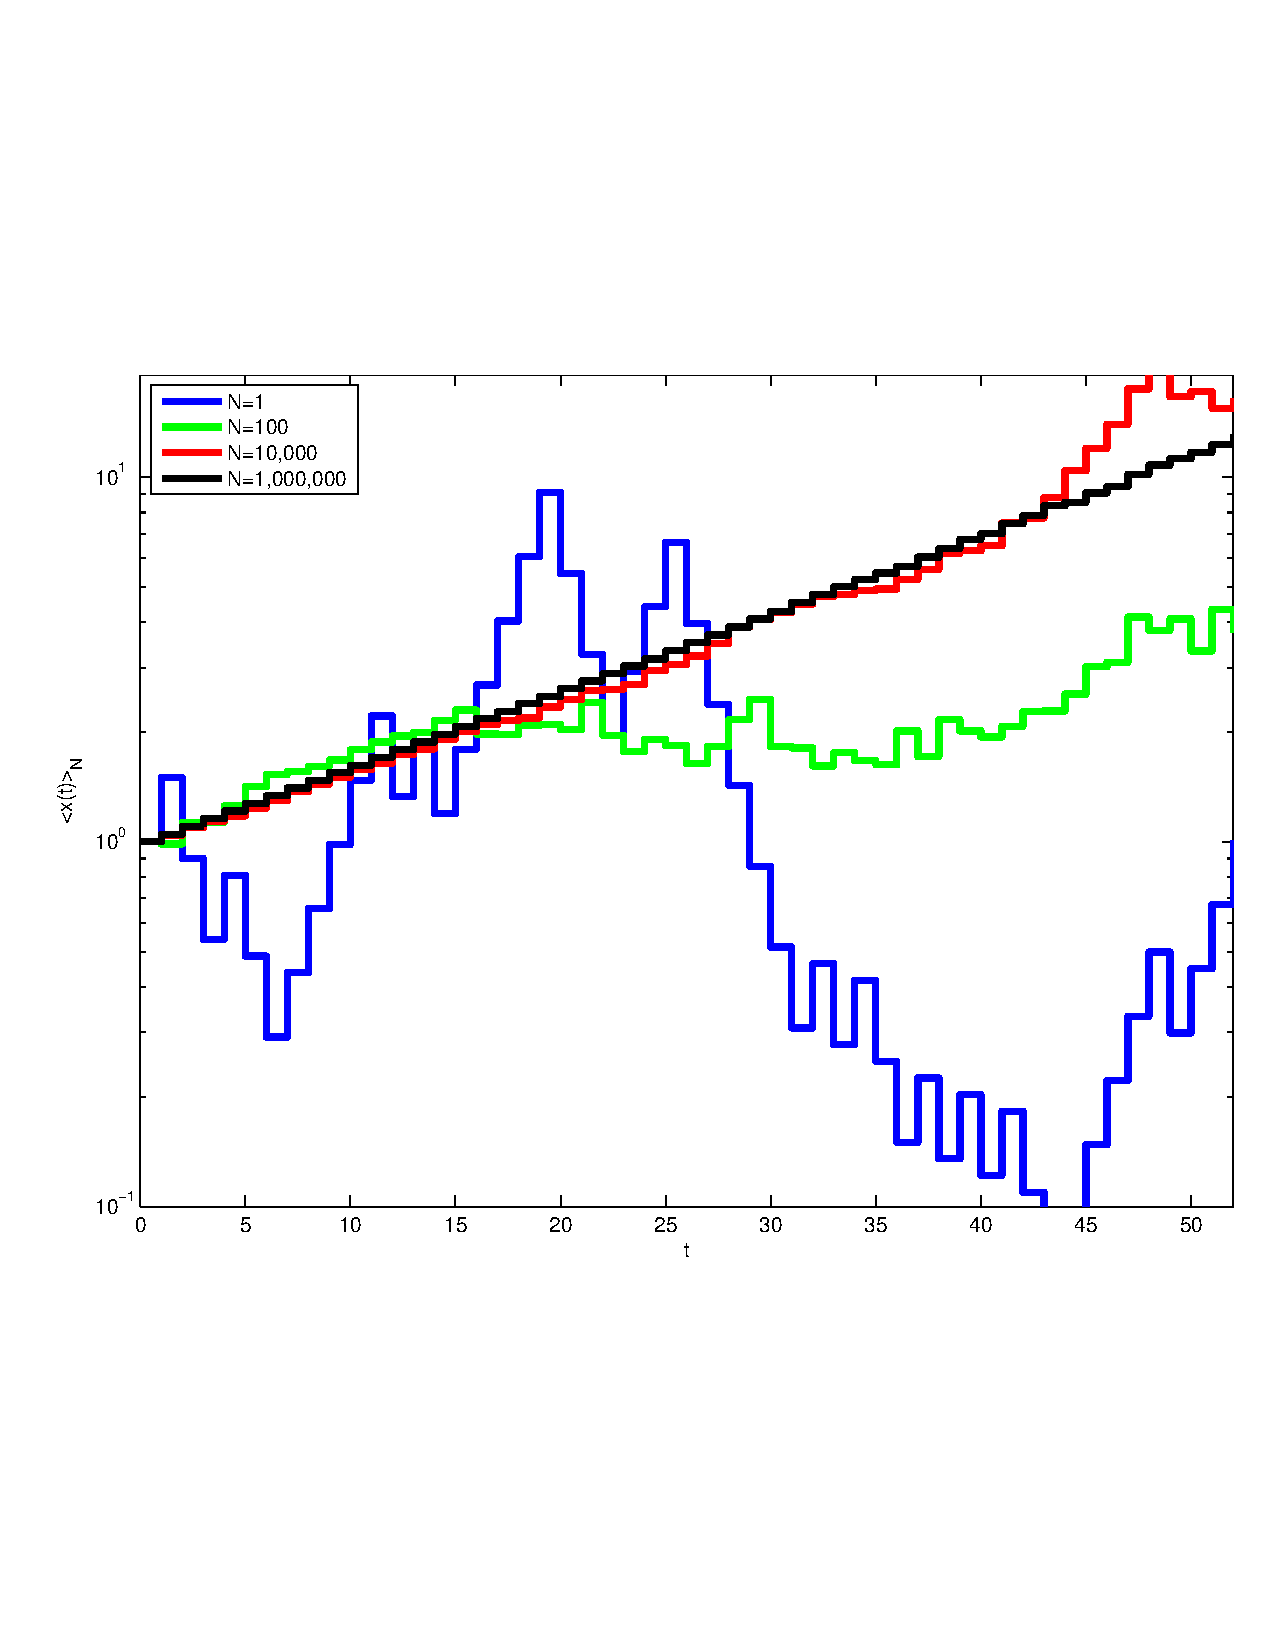
\includegraphics[width=0.8\textwidth]{./figs/fig1_2b.pdf}}
\end{picture}
\caption{Expectation value (thick light blue line) and partial ensemble averages $\ave{x(t)}_N$ for ensemble sizes $N=1, 
10^2, 
10^4, 10^6$. (A) linear scales, (B) logarithmic scales.}
\flabel{1_2}
\end{figure}


We pretended to be mathematically clueless. Of course we knew all along that the proposed game was a positive-
expectation 
value
game. Consider the expectation value of \eref{gamble}  
\be
\ave{x(t+\Delta t)}=\ave{x(t) r(t)}. 
\ee
Since $r(t)$ is independent of $x(t)$ (we draw it at random in each time step), this can be re-written as
\be
\ave{x(t+\Delta t)}=\ave{x(t)}\ave{r(t)},
\ee
wherefore we can solve recursively for
\be
\ave{x(t)}=x(0)\ave{r(t)}^t.
\ee
The expectation value of $\ave{r}$ is easily found, $\ave{r}=\frac{1}{2}\times 0.6 + \frac{1}{2}\times 1.5=1.05$. Since 
this number is greater than one, $\ave{x(t)}$ grows exponentially in time at rate 1.05 per time unit, or expressed as a 
continuous growth rate, at $\frac{1}{\Delta t}\ln(\ave{r})\approx4.9\%$ per time unit. We could now conclude that the 
case is closed: mathematics tells us that there's some risk involved, but the broad effect of subjecting our 
wealth to the rules of the game is a gain. Just wait long enough for the fluctuations to average out. 

That said, expectation values were not invented in order to 
assess whether a gamble is worth taking. Instead, they were 
developed to settle the following moral question that arises 
in a context I've always found a little contrived, but that 
didn't stop it from making a momentous contribution to 
probability theory. Imagine playing a game of dice with a 
group of gamblers. The rules of the game are simple: we 
roll the dice three times,  and whoever rolls the most points 
gets the pot to which we've all contributed equal amounts. 
We've already rolled the dice twice when suddenly the 
police burst in because they've heard of our illegal gambling ring. 
We all avoid arrest, most of us escape through the backdoor, 
and to everyone's great relief you had the presence of mind 
to grab the pot before jumping out of a conveniently located 
ground-floor window. Later that day, under the cover of dusk, 
we meet behind the old oak tree just outside of town to split 
the pot in a fair way. But hold on -- what does ``fair'' mean here?
Some of us had acquired more points than others in the first 
two rolls of the dice. Should they get more? The game was 
not concluded, so it would be fair to return to everyone his 
wager and thank our lucky stars that we weren't arrested. 
Should we split the pot in proportion to each player's points? 
The question is fundamentally moral, and there is no 
mathematical answer. But Blaise Pascal, famous for 
addressing theological questions with mathematics, put the 
problem to Fermat, and over the course of a few months' 
correspondence (the two never met in person) Fermat and 
Pascal agreed that the fair solution to the problem is the 
following. Imagine all possible outcomes of the third round 
of throws of the dice, call the number of possibilities $N$. 
Now count all those possibilities that result in player $i$ winning, 
call this $n_i$. If $M$ is the amount of money in the pot, then 
each player receives $\frac{n_i}{N}\times M$. Later researchers 
called this amout the ``mathematical expectation''  or simply 
``expectation value''. Of course we mustn't be confused by 
words, and ``expectation'' is really an unfortunate choice here
 -- no player ``expected'' to receive $M\times \frac{n_i}{N}$. 
Instead, each player expected to either receive nothing or $M$ 
depending on how his last throw of the dice would go. The 
quantity $\frac{n_i}{N}$ is called the probability of $i$ winning, 
denoted $p_i$. More generally, the expectation value of some 
quantity, $\ave{\Delta x}$ is an average of the quantity in 
different possible states of the world weighted by its 
probability, here $\ave{\Delta x}=\sum_i p_i \Delta W_i$, 
where $\Delta W=0$ if $i$ does not win, and $ \Delta 
W=M$ if $i$ does win. 


This reasoning has dominated economic theory for about 350 years now. But it is flawed. ``Just wait long enough for the 
fluctuations to average out'' -- this is not how we removed the fluctuations. We did something quite different and removed 
them by adding enough systems together and averaging over them. The implicit assumption in this argument is that waiting for a long time is equivalent to ensemble-averaging many possible paths. The question under what circumstances this equivalence holds is known as a the question of ergodicity, and it was first raised in the development of statistical mechanics by Maxwell and Boltzmann starting in the 1850s. Historically, some remarks are in order -- 1850 is about 200 years after Fermat and Pascal introduced expectation values into the study of random systems. Following the success of Newton's laws of motion the notion of ``proper science'' had become synonymous with mechanics. Mechanics had no use for probability theory, and its success of mechanics was interpreted as a sign that the world was deterministic and that sooner or later we would understand what at the time still seemed random. At that point probability theory would become obsolete. 

When Boltzmann hit upon the ingenious idea of introducing randomness into physics, to explain the laws of 
thermodynamics in terms of the underlying dynamics of large numbers of molecules, he was fighting an uphill battle. Neither molecules nor randomness were
much liked in the physics community, especially in continental Europe, right up until the publication of Einstein's 1905 
paper 
on 
diffusion.
Boltzmann had to be careful, and the question of ergodicity had to be answered -- the usefulness of probability theory 
relies 
heavily 
on expectation values, but they are technically an average over imagined trajectories of the universe. Under what 
circumstances are
they meaningful? Boltzmann gave two answers. Firstly, expectation values are meaningful when the quantity of interest 
really 
is 
an
average (or a sum) over many approximately independent systems. An average over a finite ensemble will be 
very close to the expectation value if the ensemble is large enough. Secondly, expectation values are meaningful, even if 
only a 
single
system exists, if they reflect what happens over time. In this second case Boltzmann would call a system 
ergodic\footnote{The word ``ergodic'' was coined by Boltzmann. 
He initially proposed the word "monodic'', from Greek $\mu o \nu o$ (unique)+$o\delta o \sigma$ (path) suggesting 
that a single path when followed for a sufficiently long time will explore all there is to explore and reflect what happens 
in an ensemble. The term ``ergodic'' refers to the specific system Boltzmann was considering, namely an energy 
($\epsilon \rho \gamma o \nu$) shell across which a path is being traced out.}.

As before we pretend to know nothing about mathematics and submit our game to a numerical
test, consisting of another computer simulation, in order to find out whether it is ergodic. For the system to be ergodic, 
in the most basic sense of the word, what happens on average in an ensemble has to be the same as what happens
over a long time in a single system. We make this statement precise as follows

\definition{
In these notes, an observable $A$ is called ergodic if its time average and expectation value are identical,
\be
\lim_{N\to\infty} \frac{1}{N}\sum_i^N A_i = \lim_{T\to\infty}\frac{1}{T} \int^T A(t) dt.
\ee}


 \Fref{1_3} shows another Monte Carlo simulation of your wealth, but this time
the randomness is not removed by adding more trajectories to the ensemble but by adding more time to the simulation of 
a 
single trajectory.
To capture visually what happens over a long time we will be forced to zoom out -- more time has to be represented by 
the 
same 
amount
of space on the page. In the process of this zooming-out small short-time fluctuations will diminish. Eventually 
the noise will be removed from the system just by the passage of time.

\begin{figure}[h!]
\begin{picture}(200,250)(0,0)
  \put(-50,30){(A)}
    \put(-100,-30){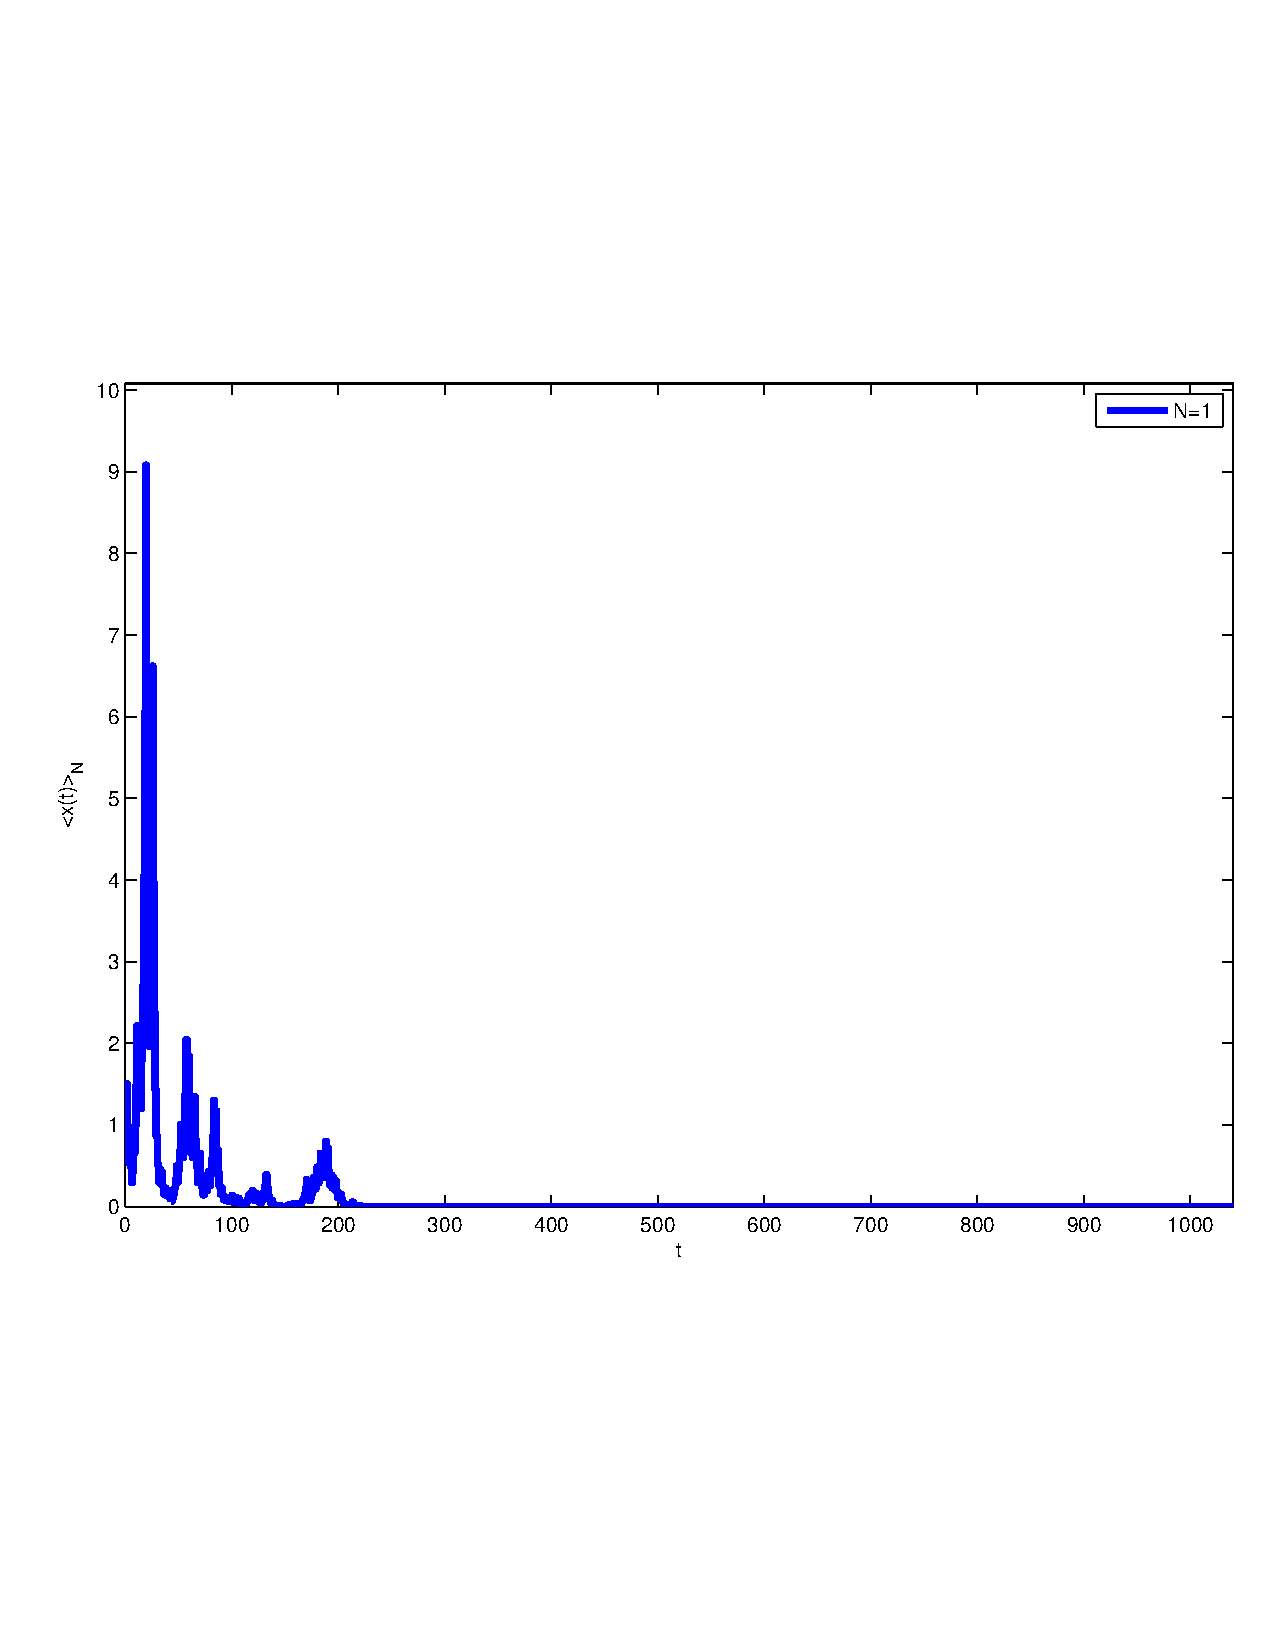
\includegraphics[width=0.8\textwidth]{./figs/fig1_3a.pdf}}
  \put(230,30){(B)}  
  \put(180,-30){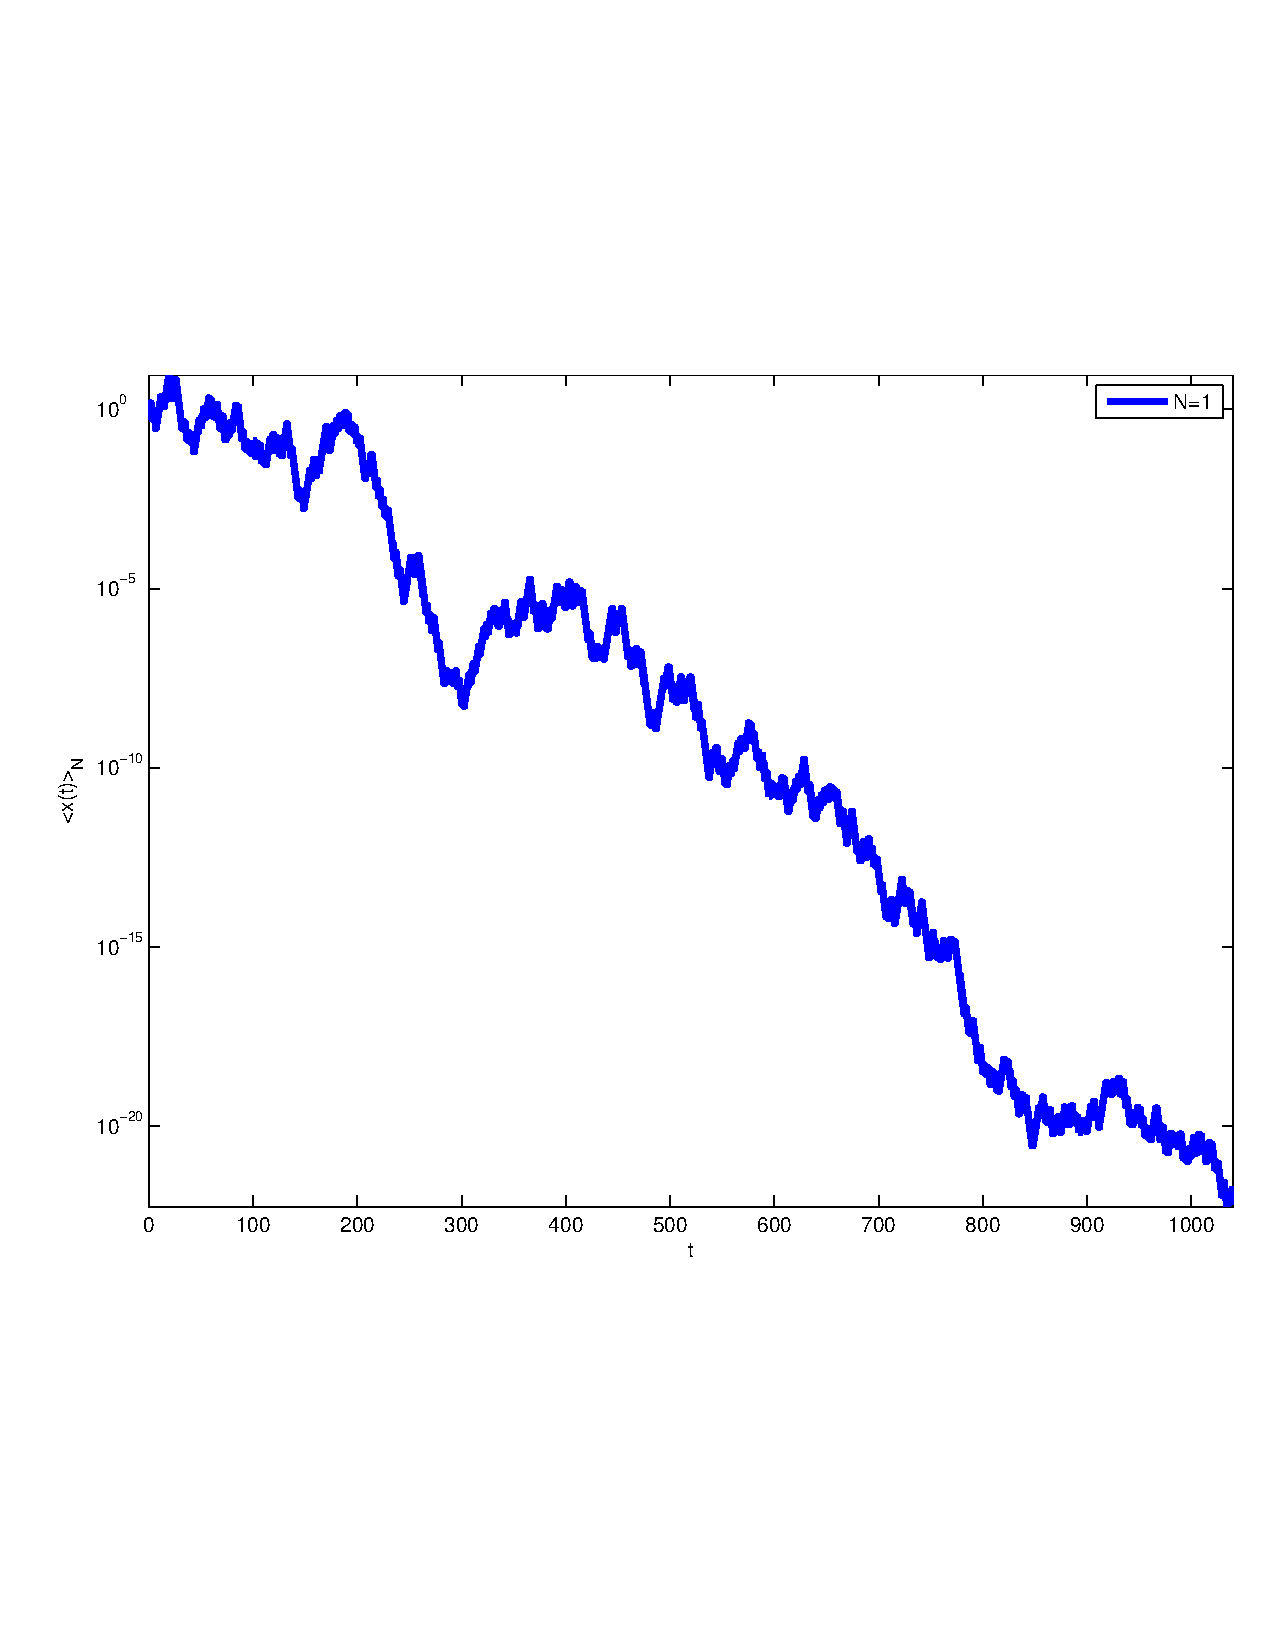
\includegraphics[width=0.8\textwidth]{./figs/fig1_3b.pdf}}
\end{picture}
\caption{Expectation value (thick light blue line) and a single trajectory over 1,040 time units, corresponding to 20 years 
in our 
setup. (A) linear scales, (B) logarithmic scales.}
\flabel{1_3}
\end{figure}

\Fref{1_3} shows unequivocally that the expectation value does not reflect what happens over 
time in a single system. Several important messages can be derived from this observation. 

\begin{enumerate}
\item
An individual whose wealth follows \eref{gamble} will make poor decisions if he uses the expectation value of wealth 
as an indication of what is likely to happen.
\item
The performance of the average (or aggregate) wealth of a large group of individuals differs systematically from 
the performance of an individual's wealth. In our case large-group wealth grows (think GDP), whereas individual wealth 
decays.
\item
For point 2 to be possible, \ie for the average to outperform the typical individual, wealth must concentrate on a 
few extremely rich individuals. The wealth of the richest individuals must be so large that the average becomes 
dominated by 
it, 
so that
the average can grow although almost everyone's wealth decays.
\end{enumerate}

To complete the discussion we compute analytically what happens in the long-time limit.
For simplicity, we set initial wealth to one, $x(t=0)=1$. The dynamic is set up such that 
wealth at time $t$ is
\be
x(t)=\prod_{t'=1}^t r(t'),
\ee
which we can split up into two products, one for each possible value of $r(t)$, which we call
$r_1$ and $r_2$. Let's denote the number of $r_1$s by $n_1$ and $r_2$s by $n_2$, 
so that
\be
x(t)= r_1^{n_1} r_2^{n_2}.
\ee
We denote by $\bar{r}$ the factor by which $x(t)$ changes when the change is computed over a long time. 
This quantity is found by taking the $t^{\text{th}}$ root of $x(t)$ and considering the long-time limit
\bea
\bar{r} &=\lim_{t\to\infty }x(t)^{1/t}\\
 &= \lim_{t\to\infty } r_1^{n_1/t} r_2^{n_2/t}.
\eea
Identifying $\lim_{t\to\infty} n_i/t$ as the probability for $r_i$ to occur this is
\be
\lim_{t\to\infty }x(t)^{1/t}= (r_1 r_2)^{1/2},
\ee
or about 0.95, \ie a number smaller than one, reflecting 
decay in the long-time limit for the individual trajectory.
The trajectory in \fref{1_3} was not a fluke: every trajectory
will decay in the long run at a rate of $(r_1 r_2)^{1/2}$ per time unit. \Fref{1_4} (B) 
compares the trajectory generated in \fref{1_3} to a trajectory decaying exactly 
at rate $\bar{r}$
and places it next to the average over a million systems for side-by-side comparison.
\begin{figure}[h!]
\begin{picture}(200,250)(0,0)
  \put(-50,20){(A)}
    \put(-100,-50){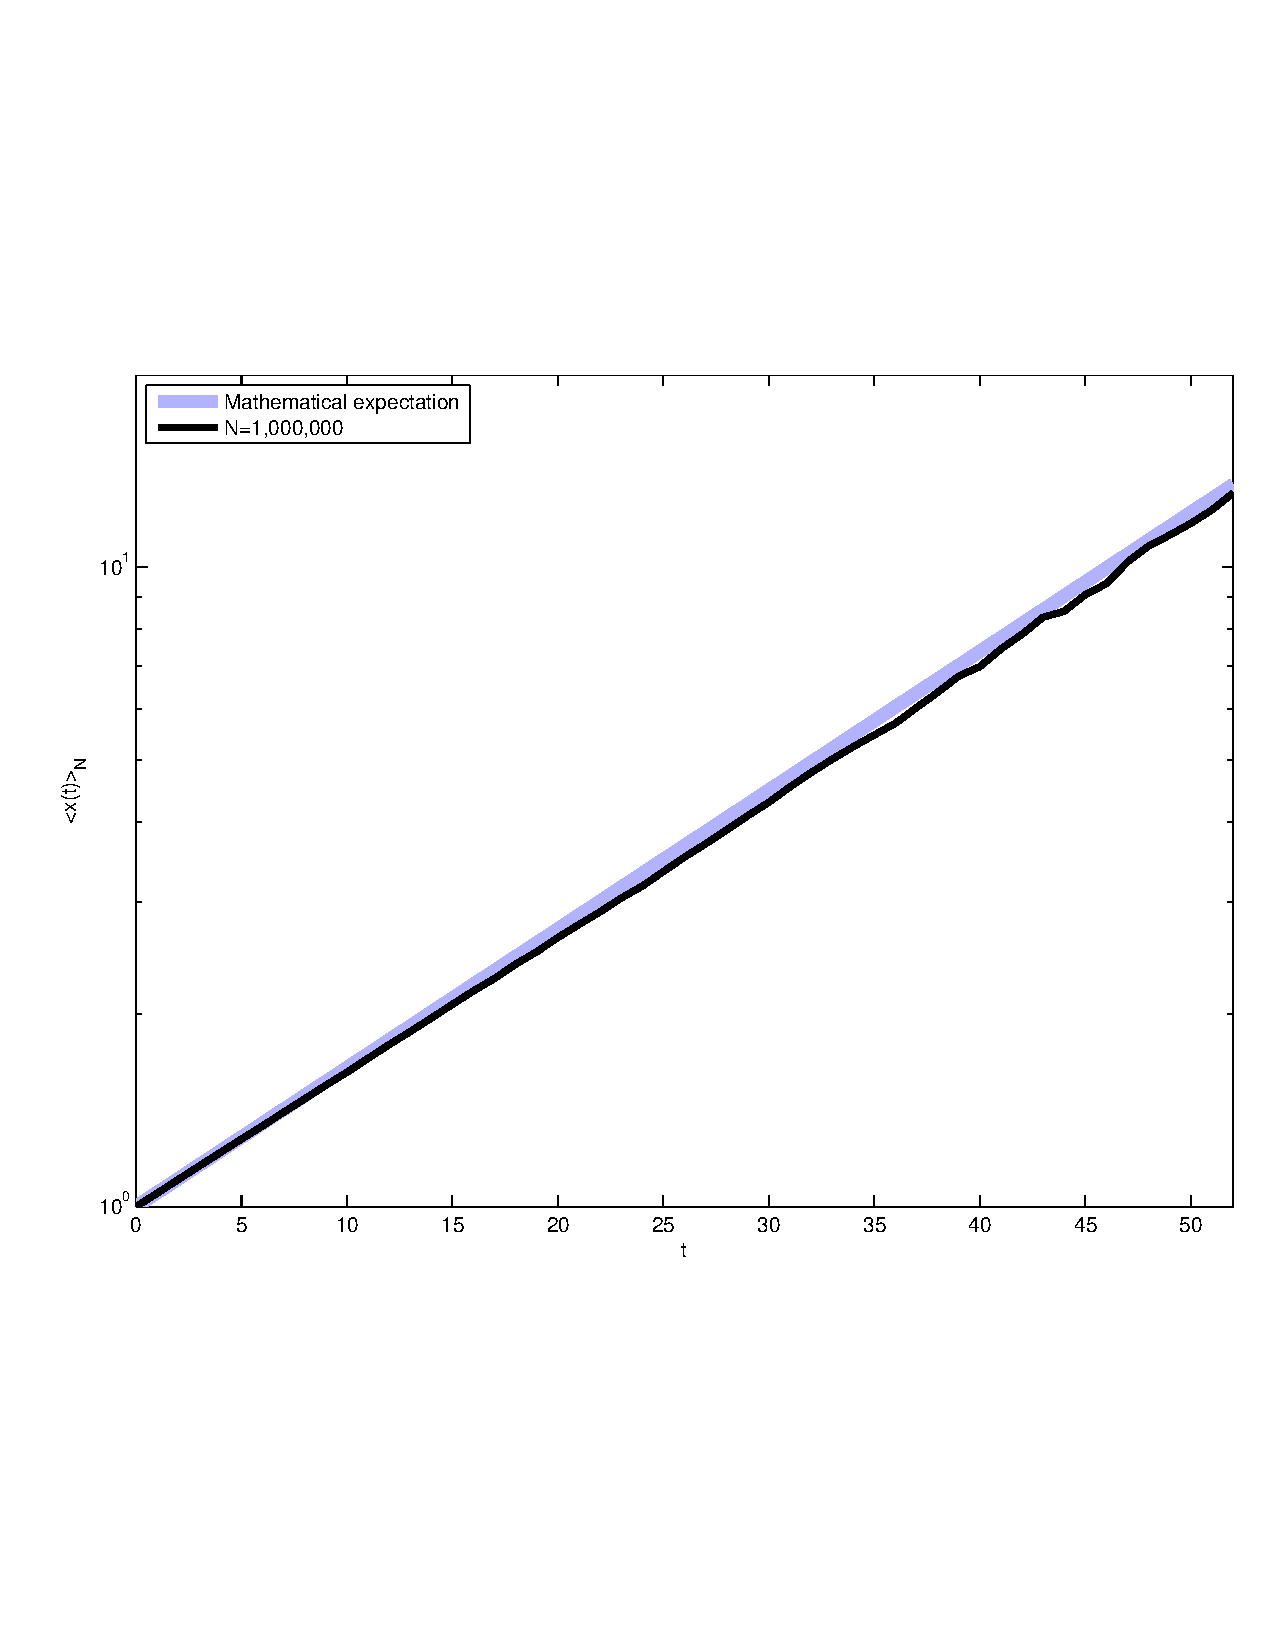
\includegraphics[width=0.8\textwidth]{./figs/fig1_4a.pdf}}
  \put(230,20){(B)}  
  \put(180,-50){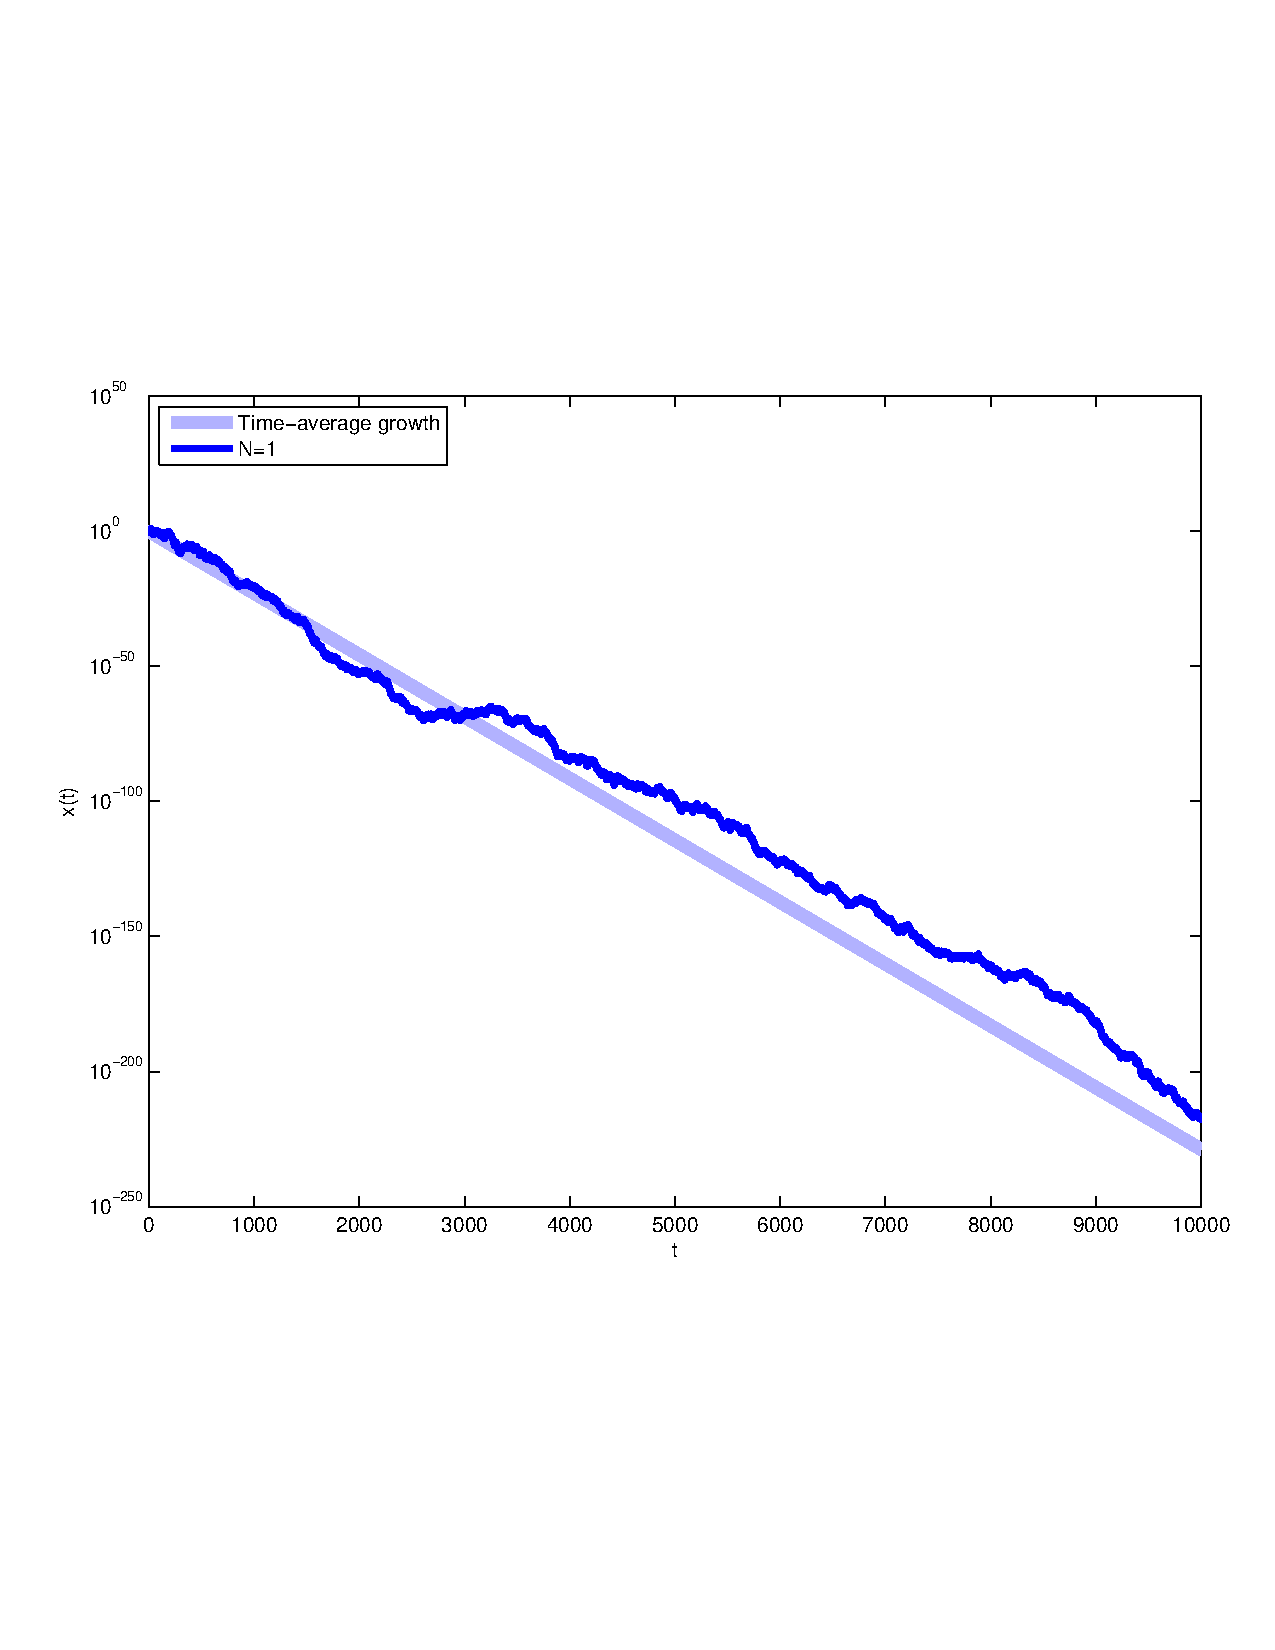
\includegraphics[width=0.8\textwidth]{./figs/fig1_4b.pdf}}
\end{picture}
\caption{(A) Finite-ensemble average for $N=10^6$ and 52 time steps, the light blue line is 
the expectation value. (B) A single system simulated for 10,000 time steps, the light blue 
line decays exponentially with the time-average decay factor $\bar{r}$ in each time step.}
\flabel{1_4}
\end{figure}

In \fref{1_4} (A) a slight discrepancy between the expectation value and the $N=10^6$ 
finite-ensemble average is visible, especially for later times. This is not coincidence --
in the long run, also the finite-ensemble average for $10^6$ systems will decay
at the time-average growth rate. A simple proof for this is in \cite{PetersKlein2013}.
Moreover, the distribution for $\ave{x(t)}_N$ is known for any $N$ and $t$ (because
it happens to be mathematically identical to the partition function of the random 
energy model, introduced and solved by Derrida \cite{Derrida1981}. We thank 
J.-P. Bouchaud for pointing this out to us).


Now we have two averages, $\ave{r}$ and $\bar{r}$, 
both of which are scalars (whereas $x(t)$ is a random variable).
Scalars have a the transitive property that is heavily relied upon in 
economic theory. Let $a_i$ be a set of scalars. Then if $a_1>a_2$ and 
$a_2>a_3$ we have $a_1>a_3$. Notice that we cannot rank random variables 
in such a way. The ``greater than'' relation, $>$,
is not defined for a pair of random variables, which is is the mathematical
way of saying that it is difficult to choose between two gambles, and it is why 
we went to the trouble of removing the randomness from the stochastic process 
$x(t)$. Removing randomness by
averaging always involves a limiting process, and results are said to hold ``with probability one''. 
In the case of $\rex$ we considered the infinite-ensemble limit, $N\to \infty$, and 
in the case of $\rt$ we considered the infinite-time limit $\lim_{t\to\infty}$. If we use the scalars 
$a_i$ to represent preferences, we can test for consistency among preferences. 
For instance, in such a model world where preferences are represented by scalars, 
the facts that ``I prefer kangaroos to Beethoven'' and ``I prefer mango chutney to kangaroos'' 
imply the fact ``I prefer mango chutney to Beethoven''. Translating back to reality, 
and individual who makes the first two statements but not the third can be
called ``irrational.'' 

Because transitivity makes for a
nicely ordered world, it is useful to find scalars to represent preferences.
We are skeptical about the attempt to map all preferences
into scalars because  the properties of mango chutney are too different, {\it qualitatively},
from the properties of Beethoven. We will restrict our analysis to money --
while the unknown nature of the amounts of money we may receive introduces
a complication, at least in the limit of no randomness we know how to compare one amount to another --
there is no qualitative differences between $\$1$ and $\$3$, only a quantitative difference. 

Both $\rex$ and $\rt$ are scalars, and both are therefore potentially powerful 
representations of preferences. Your decision whether to accept our gamble could
now be modelled as a choice between the scalar $\rt$  that corresponds to the
null-gamble (not accepting our game), namely $a_1=1$, and the scalar $\rt$ that 
corresponds to the proposed game, namely approximately $a_2=0.95$. In this 
model of your decision making you would decline the gamble because $1>0.95$.

$\rex$ and $\rt$ are two different properties of the game. $\rex$ is computed 
by taking the large-ensemble limit, $\rt$ is the long-time limit. The Victorian 
mathematician William Allen Whitworth was aware that $\rt$ is the property 
relevant for an individual deciding whether to take part in a repeated gamble, 
and used this knowledge to write an appendix  entitled ``The disadvantage 
of gambling'' to the 1870 edition of his book ``Choice and Chance'' 
\cite{Whitworth1870}. His argument, in slightly different notation, went as 
follows. Imagine that you either win or lose, with equal probability, 
an amount $x(t) \sigma \sqrt{\Delta t}$ in each round of a game. This scaling in $\Delta t$
is not arbitrarily chosen -- it would be observed if the multiplicative increment in each time interval
were the product of many independent smaller multiplicative 
increments, $\ln r=\sum_i \ln r_i \delta t$. In the long run, positive and 
negative changes will occur equally frequently, and to determine
the overall effect we just need to consider the effect of a positive and a negative change
in a row. We take the square root of this factor to determine what happens -- in the time average 
-- in a single round. This will be 
\be
[(1+\sigma \sqrt{\Delta t})(1-\sigma \sqrt{\Delta t})]^{1/2}= (1-\sigma^2 \Delta t)^{1/2}
\ee
Letting $\Delta t$ become infinitesimal we replace it by $dt$, and 
the first term in a Taylor expansion becomes exact. We find
\be
\left[(1+\sigma \sqrt{\Delta t})(1-\sigma \sqrt{\Delta t})\right]^{1/2}\to 1-\frac{\sigma^2}{2} dt.
\ee
We choose this notation (also in \secref{Geometric_Brownian}) to anticipate \Ito's 
work of 1944 that is now the basis of much of financial mathematics.

Whitworth was arguing against a dogma of expectation values of wealth, that had 
been established almost immediately following Fermat and Pascal's work. He 
hoped to show mathematically that gambling is not a good idea, and was a 
proponent of the notion that commerce should and does
consist of mutually beneficial interactions rather than one winner and one loser. 
In the end his voice was not heard in the economics
or mathematics communities. He quit mathematics to become a priest at All Saints Church
in London's Margaret Street, only a 22 minute stroll away from the London 
Mathematical Laboratory, according to Google.
\begin{figure}[h!]
\begin{picture}(200,250)(0,0)
  \put(0,0){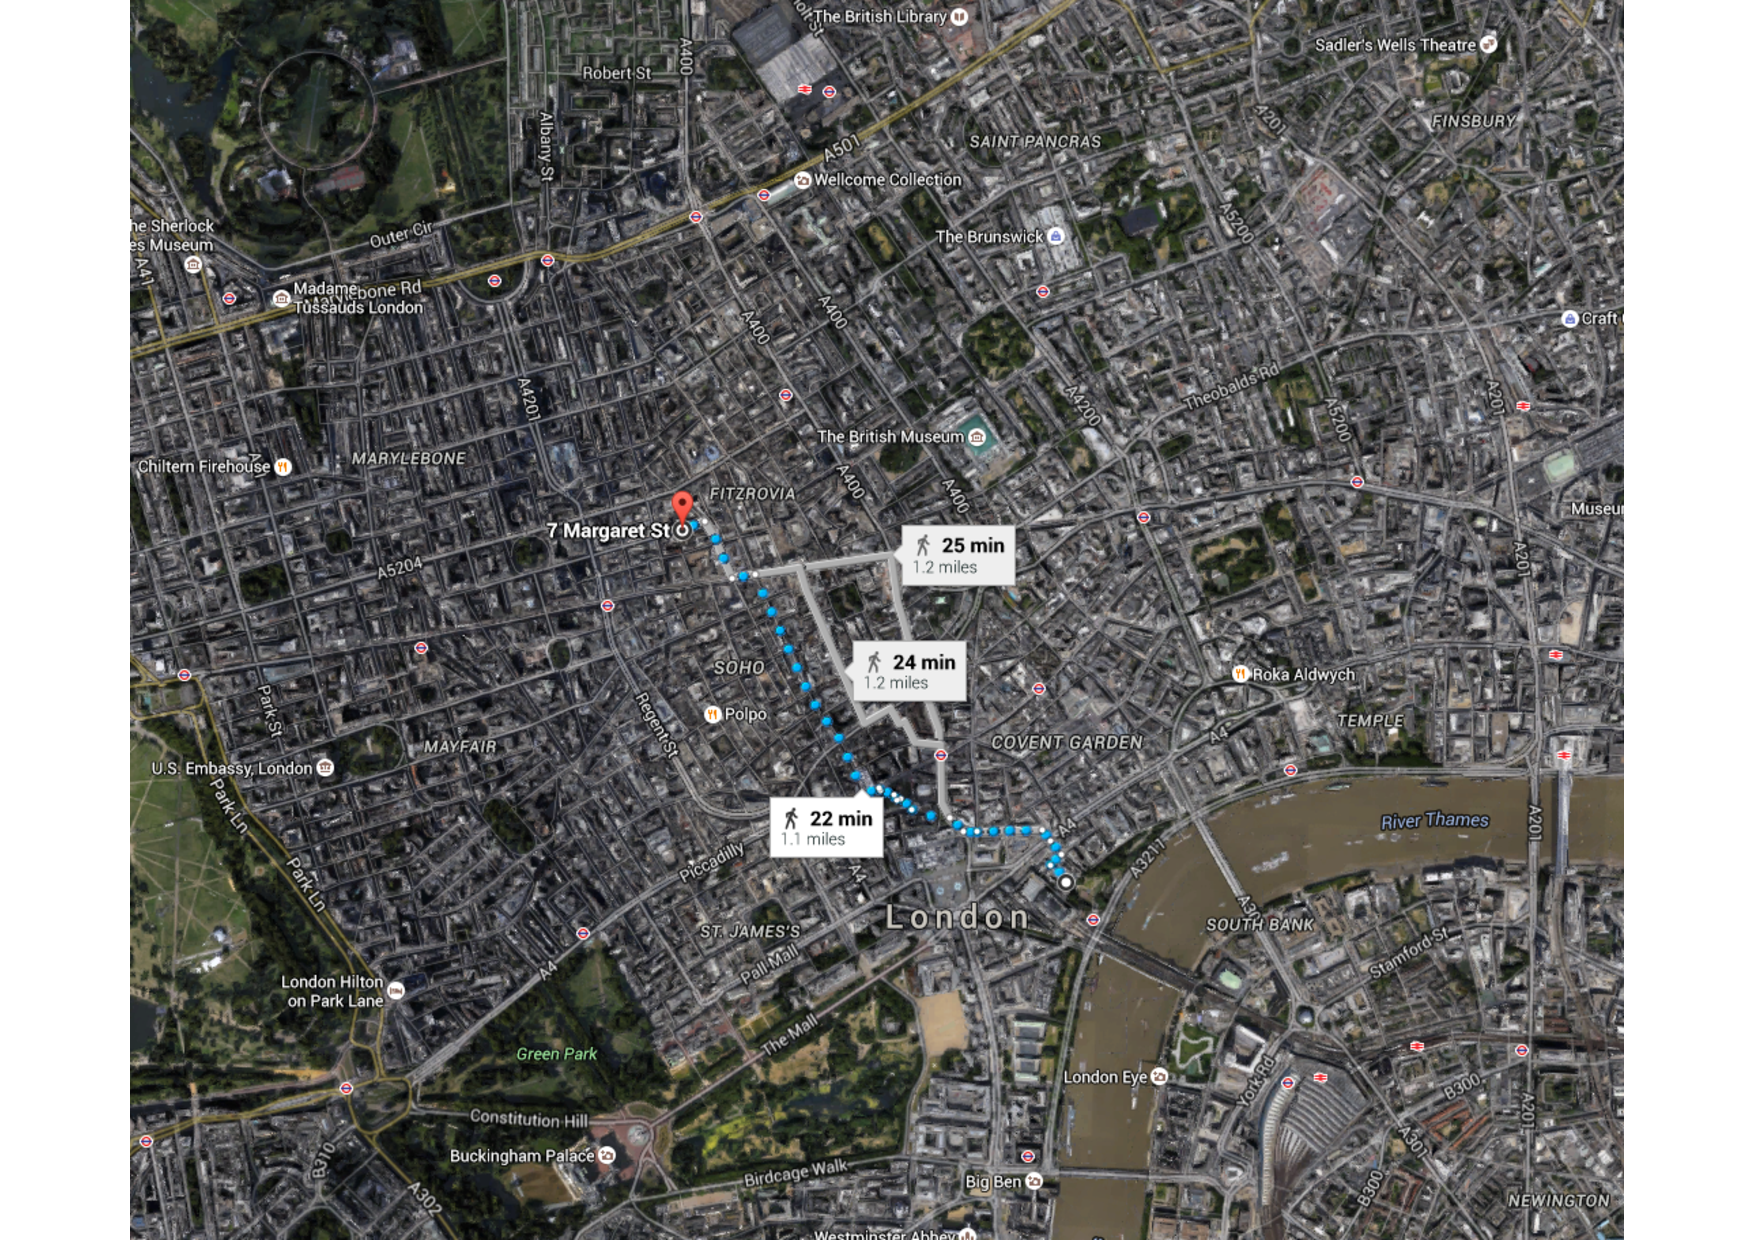
\includegraphics[width=1\textwidth]{./figs/all_saints.pdf}}
\end{picture}
\caption{Location of All Saints Church and the London Mathematical Laboratory.}
\flabel{all_saints}
\end{figure}


\subsection{Rates}
\seclabel{Rates}
At this point it is helpful to discuss the notion of a rate of change and the notion of stationarity. 
To do this properly let's think about the basic task of science. This may be described as the 
search for stable structure. More precisely science attempts to build models of the world 
whose applicability necessarily varies from one specific case to another, but does not 
vary over time. This does not mean that the models do not describe change, but the way 
in which they describe change does not change. Something, some property of the model 
remains unchanged. This property is often somewhat grandiosely called a law of nature.

Newton's laws are a good illustration of this. They are part of mechanics, meaning that they
are an idealized mathematical model of the behavior of positions, velocities, and masses. 
For instance, Newton's second law states that the mass multiplied by the rate of 
change of the rate of change of its position equals the force. The law is an unchanging 
law about positions, but it does not say that positions don't change, it doesn't even say 
that rates of change of positions don't change. It does say that the rate of change of the 
rate of change of a position remains unchanged so long as the force and the mass 
remain unchanged.

Our game is a prescription of changes, but in contrast to Newton's laws it is a stochastic
prescription. We're fundamentally interested in changes -- we want to know 
whether we're winning or losing -- but to judge stationarity of changes we will have to look at
the stochastic law, \ie the probability distribution, that describes changes. If this distribution
is stationary then we have found an observable that is stable.

Under the rules of the game wealth $x(t)$ is not stable, it's a different 
random variable for each $t$. But the stochastic law according to which the wealth 
changes is stable. Can this be expressed as a rate of change? Clearly, 
the stochastic law in \eref{law} that describes $\frac{\Delta x(t)}{\Delta t}$ depends on $x(t)$ because
changes in $x(t)$ are proportional to $x(t)$, so the rate of change of $x(t)$ is no good. 
Ideally we would find a rate of change of wealth whose probability law is stationary. 
We want the rate of change of wealth because that's ultimately what we're interested in. 
If this were stationary then its expectation value would be temporally meaningful: 
in each time step we would add an amount that's drawn from a stationary distribution; 
$x(t)$ would just be the sum of these increments, and the expectation value of the 
increment would converge to the long-time average.

But alas! This is not the case. $\frac{\Delta x}{\Delta t}$ is not stationary. But we can use the following
clever idea: we wanted to know whether $x(t)$ is growing or shrinking in the long run, and we wanted
to see that by computing the expectation value of a rate of change, meaning we want the rate
of change to be ergodic. Our first attempt failed, but
if we found a monotonically increasing function of $x(t)$ to be growing over time, then 
we would know that $x(t)$ is growing as well. In other words, 
as long as we can find a monotonically increasing function $f(x)$ whose increments 
$\frac{\Delta f(x)}{\Delta t}$ are stationary, then we can also find out whether $x(t)$ grows
in the long run by computing the expectation value of $\frac{\Delta f(x)}{\Delta t}$.

Section~\ref{The_game} was an illustrative example that was designed to weaken any pre-conceived
notions the reader may have. But the analysis of the problem was haphazard. We want a
systematic way of analyzing any type of game. Here it is
\begin{enumerate}
\item
Given the stochastic process $x(t)$
\item
Find a monotonically increasing function $f[x(t)]$ such that $\frac{\Delta f[x(t)]}{\Delta t}$ 
are independent instances of a stationary random variable.
\item
Compute the expectation value of $\frac{\Delta f[x(t)]}{\Delta t}$. If this is positive then $x(t)$
grows in the long run, if it is negative then $x(t)$ decays.
\end{enumerate}

For our game the function $f(x)$ is the logarithm. We repeat: this is a function that satisfies 
two conditions. Firstly, it is monotonically increasing in $x(t)$. Secondly its rate of change 
$\frac{\Delta f[x(t)]}{\Delta t}$ is stationary (its probability distribution does not depends on $t$).

Firstly, the logarithm is a monotonically increasing function of its argument.

Secondly, the game is defined by a set of factors of increase in $x(t)$, \eref{gamble}. Therefore, the quantity
$\frac{x(t+\Delta t)}{x(t)}$ has a stationary distribution. The function whose change in response to a change 
of its argument is the same as the function of the ratio of the two values of the argument is the logarithm, \ie
only the logarithm satisfies
\be
f[x(t+\Delta t)]-f[x(t)]=f\left[\frac{x(t+\Delta t)}{x(t)}\right].
\ee

We conclude that for multiplicative dynamics, \ie if $\frac{x(t+\Delta t)}{x(t)}$ is stationary, the expectation 
value of the rate of change of the logarithm of $x(t)$ determines whether the game is long-term profitable 
for an individual.

\subsection{Brownian motion}
In the previous section we established that the discrete increments of the logarithm of 
$x$, which we called $f$, are stationary and independent in our game. A quantity for which this is the case performs a 
random 
walk.
Indeed, the blue line for a single system in \fref{1_2} (B) shows 52 steps of a random walk trajectory.
Random walks come in many forms -- in all of them $f$ changes discontinuously by an amount 
$\Delta f$ drawn from a stationary distribution, in time steps $\Delta t$ that are themselves 
drawn from a stationary distribution.

We are interested only in the simple case where $f$ changes at regular intervals, $\Delta t, 2\Delta t ...$. For 
the distribution of increments we only insist on the existence of the variance, meaning we insist that 
$\var(\Delta f)=\ave{\Delta f^2}-\ave{\Delta f}^2$ be finite. The change in $f$ after a long time is then the sum 
of many stationary independent increments, 
\be
f(t+T\Delta t)-f(t)=\sum_i^T \Delta f_i
\ee
The Gaussian central limit theorem tells us that such a sum, properly rescaled, will be 
Gaussian distributed
\be
\lim_{T\to\infty} \frac{1}{\sqrt{T}}\sum_i^T \Delta f_i \sim \mathcal{N}(\ave{\Delta f}, \var(\Delta f)),
\ee
where we call $\ave{\Delta f}$ the drift term. The logarithmic change in the long-time limit that was 
of interest to us in the analysis of the coin toss game is thus Gaussian distributed. Imagine 
simulating a single long trajectory of $f$ and plotting it on paper. The amount of time that has 
to be represented by a fixed length of paper increases linearly with the simulated time
because the paper has a finite width to accommodate the horizontal axis. 
If $\ave{\Delta f} \neq 0$ then the amount of variation in $f$ that has to be represented by a fixed
amount of paper also increases linearly with the simulated time. However, the departures of $f(t)$ from
its expectation value $t \ave{\Delta f}$ only increase as the square-root of $t$. Thus, the 
amount of paper-space given to these departures scales as $t^{-1/2}$, and for very long simulated
times the trajectory will look like a straight line on paper.

In an intermediate regime, fluctuations will still be visible but they will also be Gaussian distributed. 
In this regime it is often easier to replace the random walk model with the corresponding continuous
process. That process is called Brownian motion. We define Brownian motion as follows:

\definition{If a stochastic process has continuous paths and is distributed according to 
$\mathcal{N}(\mu t, \sigma t)$ then it is a Brownian motion.}

The process can be defined in different ways. Another illuminating definition is this:

\definition{If a stochastic process is continuous, with stationary independent increments, then the process is a Brownian 
motion.}

We quote from \cite{Harrison2014}: ``This beautiful theorem shows that Brownian motion can actually be defined
by stationary independent increments and path continuity alone, with normality following as a consequence 
of these assumptions. This may do more than any other characterization to explain the significance of 
Brownian motion for probabilistic modeling.''

Indeed, BM is not just a mathematically rich model but also -- due to its emergence through the Gaussian 
central limit theorem -- a very universal model, \ie it is a good description of what happens over long times 
in many other models. BM is a process with two parameters, $\mu$ and $\sigma$.
It can be written as a stochastic differential equation
\be
dx=\mu dt + \sigma dW
\elabel{BM_dx}
\ee
where $dW$ is a Wiener increment. The Wiener increment can be defined by its distribution and correlator, 
\be
dW \sim \mathcal{N}(0,dt),\\
\ave{dW(t) dW(t')}=dt \delta(t,t'),
\ee
where $\delta(t,t')$ is the Kronecker delta -- zero if its two arguments differ ($t\neq t'$), and one if 
they are identical ($t=t'$).
\footnote{Physicists often write $dW=\eta dt$, where $\ave{\eta}=0$ and 
$\ave{\eta(t) \eta(t')}=\delta(t-t')$, in which case $\delta(t-t')$ is the Dirac 
delta function, defined by the integral $\int_{-\infty}^{\infty} f(t) \delta(t-t') dt=f(t')$. Because of its singular
nature ($\eta(t)$ does not exist (``is infinite''), only its integral exists) it can be difficult to develop
an intuition for this object, and we prefer the $dW$ notation. }
In simulations Brownian motion paths can be constructed from a discretized version of \eref{BM_dx}
\be
f(t+\Delta t)=f(t)+ \mu \Delta t + \sigma \sqrt{\Delta t} \xi_t,
\ee
where $\xi_i$ are instances of a standard normal distribution.

BM itself is not stationary, which makes it non-ergodic according to our definition. This is easily seen
by comparing time average and expectation value
\be
\ave{x}_N \sim \mu t+\mathcal{N}(0, t/N)
\elabel{ens}
\ee

\be
\bar{x}_t \sim \mu t/2 + \sigma \mathcal{N}(0, t/3)
\elabel{tim}
\ee

The expectation value, \ie the limit $N\to\infty$ of \eref{ens}, converges to $\mu t$ with probability 
one, so it's not stationary, it depends on time, and it's unclear what to compare it to. Its 
limit $t\to\infty$ for finite $N$ does not exist. 

The time average, the limit $t\to\infty $ of \eref{tim} diverges unless $\mu=0$, but even with 
$\mu=0$ the limit is a random variable with diverging variance -- something whose density 
is zero everywhere. In no meaningful sense do the two expressions converge to the same 
scalar in the relevant limits.

Clearly, BM, whose increments are independent and stationary, is not ergodic. That doesn't make it
unmanageable or unpredictable -- we know the distribution of BM at any moment in time. But the non-ergodicity
has surprising consequences of which we mention one now. We already mentioned
that if we plot a Brownian trajectory on a piece of paper it will turn into a straight line for long enough
simulation times. This suggests that the randomness of a Brownian trajectory becomes irrelevant
under a very natural rescaling. Inspired by this insight let's hazard a guess as to what 
the time-average of zero-drift BM might be. The simplest form of zero-drift BM starts at zero, $f(0)=0$
and has variance $\var(f(t))=t$ (this process is also known as the Wiener process). The process is 
known to be recurrent -- it returns to zero with probability one in the long-time limit. We would
not be mad to guess that the time average of zero-drift BM,
\be
\bar{f}=\lim_{t\to\infty} \frac{1}{t}\int_0^t dt' f(t')
\ee
will converge to zero with probability one. But we would be wrong. Yes, the process has no drift, and
yes it returns to zero infinitely many times, but the long-time limit of its time average is not a delta function at zero.
It is, instead normally distributed with infinite variance according to the following limit
\be
\bar{f}\sim \lim_{t\to\infty} \mathcal{N}(0,t/3).
\ee
Averaging over time, in this case, does not remove the randomness. A sample 
trajectory of the time average is shown in \fref{1_6}. In the literature the process 
$\frac{1}{t}\int_0^t dt' f(t')$ is known as the ``random acceleration process'' \cite{Burkhardt2007}.

\begin{figure}[h!]
\begin{picture}(200,210)(0,0)
    \put(-0,-80){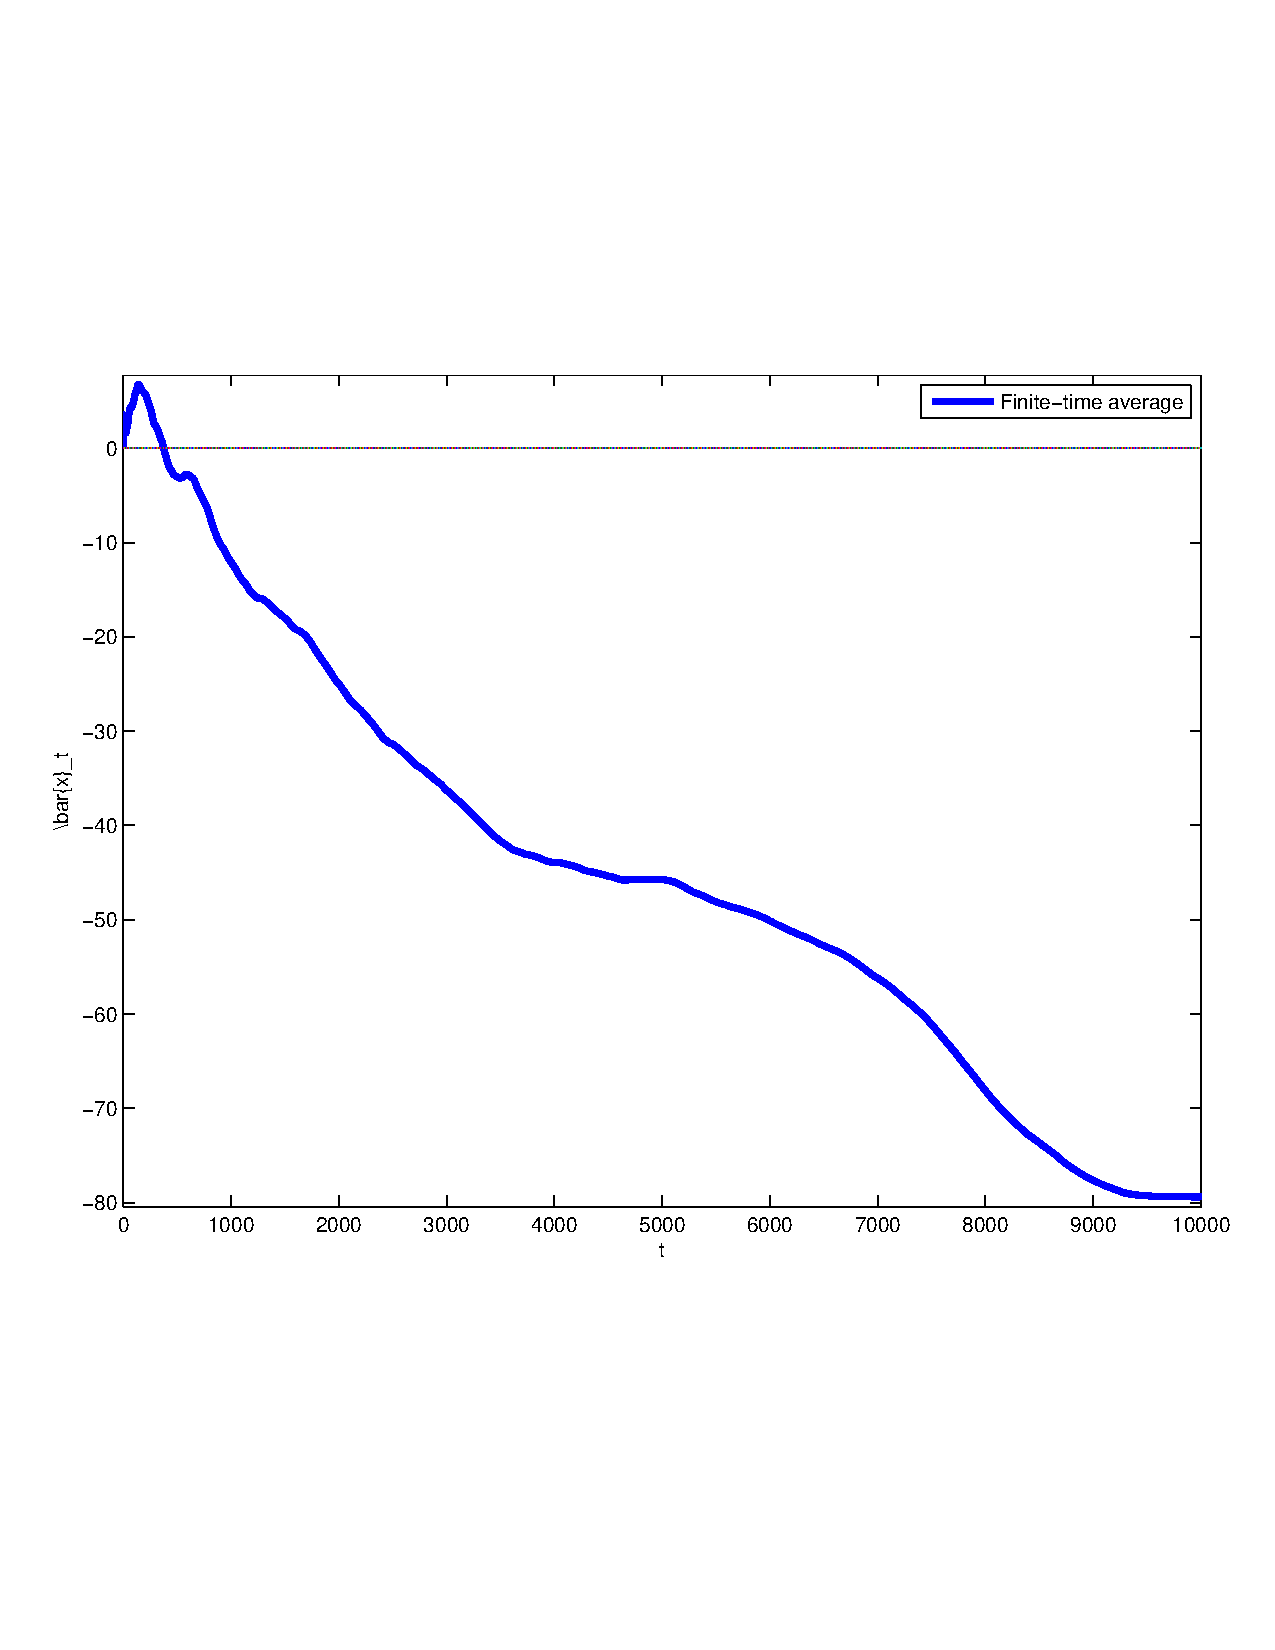
\includegraphics[width=0.8\textwidth]{./figs/fig1_5.pdf}}
\end{picture}
\caption{Trajectory of the finite-time average of a zero-drift Brownian motion. The time average 
does not converge to some value with probability one, but is instead distributed according to 
$\mathcal{N}(0,t/3)$ for all times. It is the result of integrating a BM; integration is a smoothing
operation, and as a consequence the trajectories are smoother (unlike a BM trajectory, they 
are differntiable).}
\flabel{1_6}
\end{figure}


\subsection{Geometric Brownian motion}
\seclabel{Geometric_Brownian}
\definition{If the logarithm of a quantity performs Brownian motion, the quantity itself performs ``geometric Brownian 
motion.''}

While in the previous chapter $f(x)=\ln(x)$ performed Brownian motion, $x$ itself performed geometric Brownian motion.
The change of variable from $x$ to $\ln(x)$ is trivial in a sense but it has interesting consequences. 
It implies, for instance, that 
\begin{itemize}
\item $x(t)$ is log-normally distributed
\item increments in $x$ are neither stationary nor independent
\item $x(t)$ cannot become negative 
\item the most likely value of $x$ (the mode) does not coincide with the 
expectation value of $x$. The median is the same as the mode.
\end{itemize}
The log-normal distribution is not symmetric, unlike the Gaussian 
distribution. 

Again, it is informative to write geometric Brownian motion as a stochastic differential equation. 
\be
dx=x(\mu dt+ \sigma dW).
\elabel{GBM_c}
\ee
Trajectories for GBM can be simulated using the discretized form
\be
\Delta x=x(\mu \Delta t+ \sigma \sqrt{\Delta t} \xi_t),
\elabel{GBM_d}
\ee
where $\xi_t \sim \mathcal{N}(0,1)$ are instances of a standard normal variable. In such simulations
we must pay attention that the discretization does not lead to negative values of $x$. This 
happens if the expression in brackets is smaller than $-1$ (in which case $x$ changes negatively by more than itself).
To avoid negative values we must have $\mu \Delta t + \sigma \sqrt{\Delta t} \xi_t>-1$, or 
$\xi <\frac{1+\mu\Delta t}{\sigma \sqrt{\Delta t}}$. As $\Delta t$ becomes large it becomes more likely for
$\xi$ to exceed this value, in which case the simulation fails. But $\xi_t$ is Gaussian distributed, meaning
it has thin tails, and choosing a sufficiently small value of $\Delta t$ makes these failures essentially impossible.

On logarithmic vertical scales, GBM looks like BM, and we've already seen some examples. 
But it is useful to look at a trajectory of GBM on linear scales to develop an intuition for this important process.
\begin{figure}[h!]
\begin{picture}(200,210)(0,0)
    \put(-0,-80){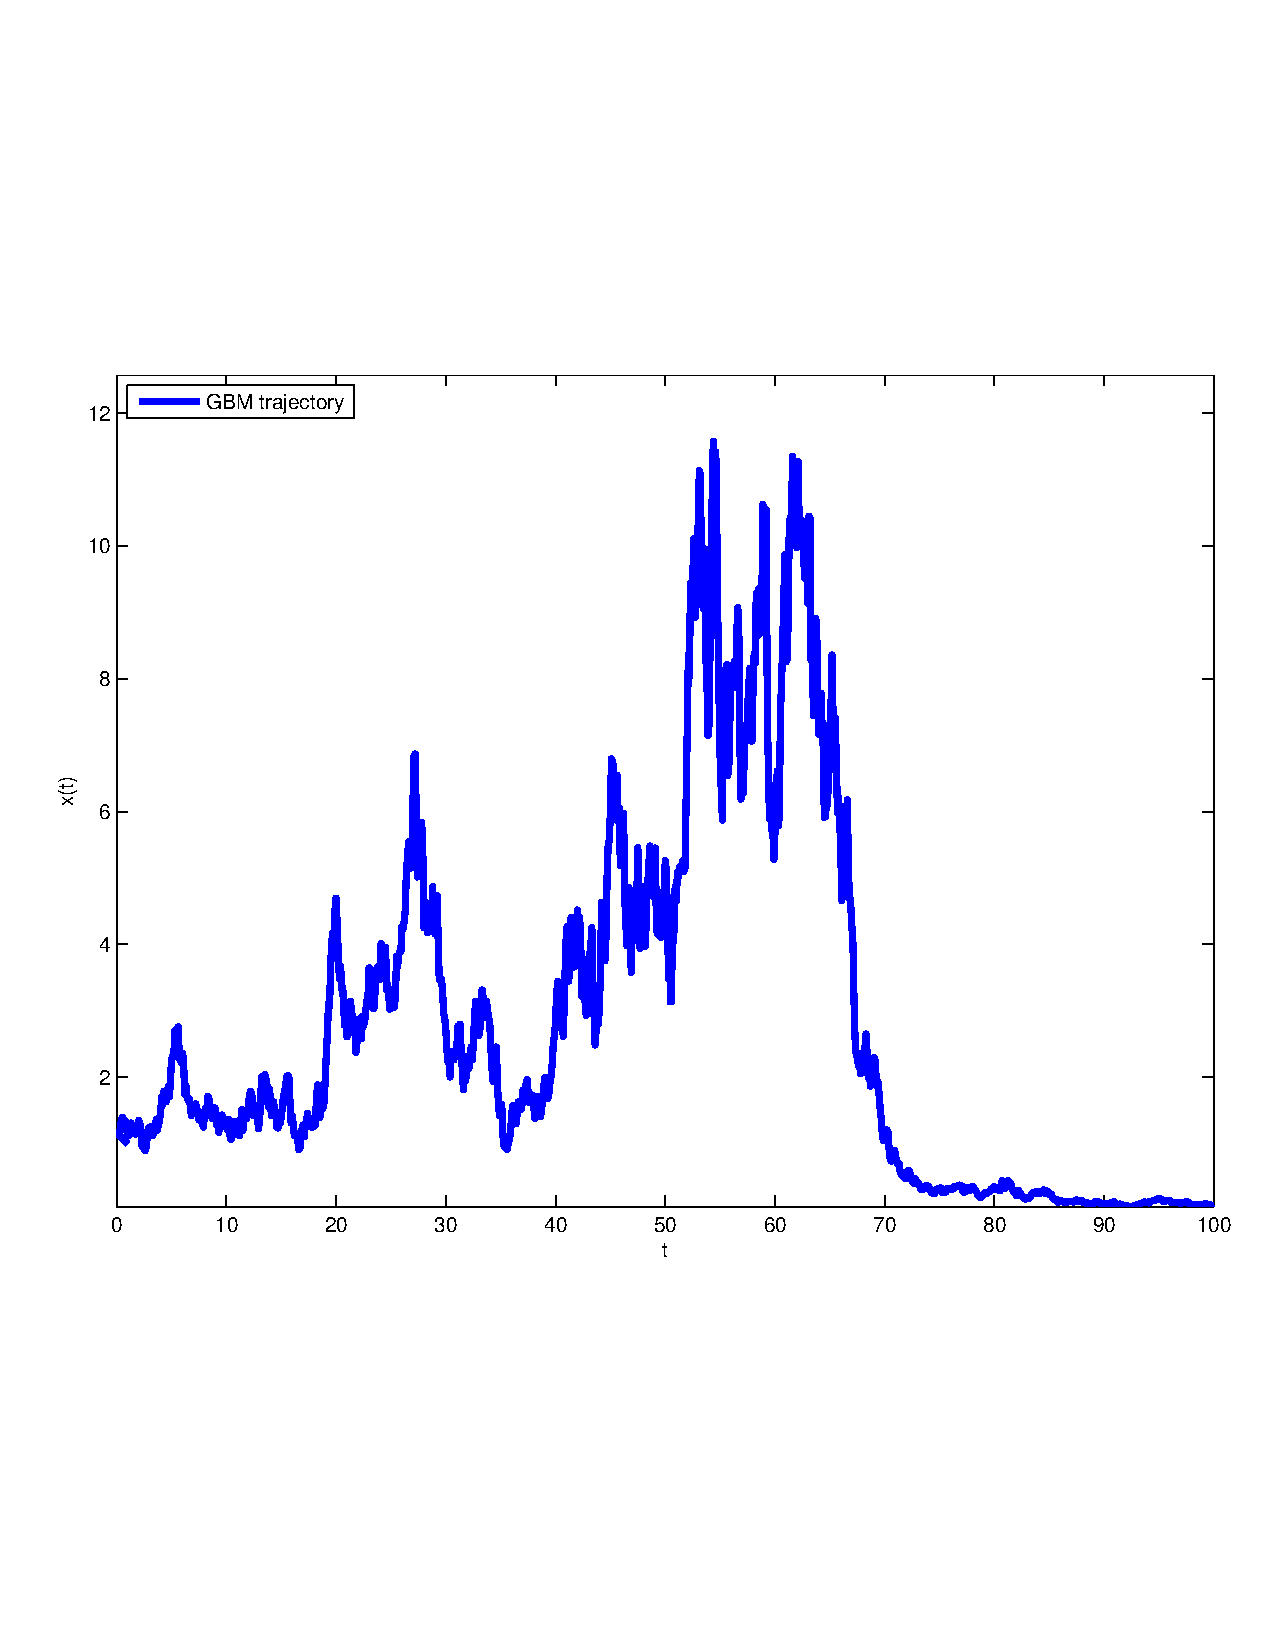
\includegraphics[width=0.8\textwidth]{./figs/fig1_6.pdf}}
\end{picture}
\caption{Trajectory of a GBM. The trajectory seems to know about its history -- for instance, unlike for BM, it is difficult to 
recover
from a low value of $x$, and trajectories are likely to get stuck near zero. Occasional excursions are characterised
by large fluctuations. Parameters are $\mu=0.05$ per time unit and $\sigma=\sqrt{2 \mu}$, corresponding to zero 
growth rate in the long run. It would be easy to invent a story to go with this (completely random) trajectory --
perhaps something like  ``things were going well
in the beginning but then a massive crash occurred that destroyed morale.''}
\flabel{1_7}
\end{figure}

The basic message of the game from \secref{The_game} is that we may obtain different values for growth rates, depending on
how we average them -- an expectation value is one average, a time average is quite a different thing. The game 
itself is sometimes called the multiplicative binomial process \cite{Redner1990}, we thank S. Redner for 
pointing this out to us. GBM is the continuous version of the multiplicative binomial process, and it shares the
basic feature of a difference between the growth rate of the expectation value and time-average growth.

The expectation value is easily computed -- the process is not ergodic, but that does not mean we cannot
compute its expectation value. Its expectation value changes in time, which is not possible for an ergodic 
observable but we can easily compute it. To compute the expectation value we simply take expectations of both sides of
\eref{GBM_c},
\bea
\ave{dx}&=\ave{x(\mu dt+ \sigma dW)}\\
&=d\ave{x}=\ave{x} \mu dt.
\eea
This differential equation has the solution 
\be
\ave{x(t)}=x_0\exp(\mu t),
\ee
which determines the growth rate of the expectation value as 
\be
g_{\ave{}}=\mu.
\ee

As we know this growth rate is different from the growth rate that materializes with probability 1 in the long run. 
Computing this time-average growth rate is only slightly more complicated. 
We will follow this plan: consider the discrete process \eref{GBM_d} and compute the changes in the logarithm of $x$, 
then we will let
$\Delta t$ become infinitesimal and arrive at the result for the continuous process. We know $\Delta \ln(x(t))$
to be ergodic, wherefore we will proceed to take its expectation value to compute the time average 
of the exponential growth rate of the process. 

The change in the logarithm of $x$ in a time interval $\Delta t$ is
\bea
\ln x(t+\Delta t) - \ln x(t) &=\ln [x(1+\mu \Delta t+ \sigma \sqrt{\Delta t} \xi_t)] - \ln x(t)\\
&=\ln x + \ln (1+\mu \Delta t+ \sigma \sqrt{\Delta t} \xi_t) - \ln x(t)\\
&=\ln (1+\mu \Delta t+ \sigma \sqrt{\Delta t} \xi_t),
\eea
which we Taylor-expand as $\ln(1+ \text{something small})$ because we will let $\Delta t$ become small.
Expanding to second order,
\be
\ln x(t+\Delta t) - \ln x(t) =\mu \Delta t+ \sigma \sqrt{\Delta t} \xi_t - \frac{1}{2} \left(\mu \sigma \Delta t^{3/2}\xi_t+
\sigma^2\Delta t 
\xi_t^2\right)+o(\Delta t^2),
\ee
using ``little-o notation'' to denote terms that are of order $\Delta t^2$ or smaller. Finally, because
$\Delta \ln x(t)$ is ergodic, by taking the expectation value of this equation we find the
time average of $\Delta \ln x(t)$
\be
\ave{\ln x(t+\Delta t) - \ln x(t)} =\mu \Delta t- \frac{1}{2} \left(\mu^2\Delta t^2+\sigma^2\Delta t \right)+o(\Delta t^2).
\ee
Letting $\Delta t$ become infinitesimal the higher-order terms in $\Delta t$ vanish, and we find
\be
\ave{\ln x(t+dt) - \ln x(t)} =\mu dt- \frac{1}{2} \sigma^2 dt
\ee
so that the time-average growth rate is
\be
\gt=\frac{d \ave{\ln x}}{dt}=\mu - \frac{1}{2} \sigma^2.
\ee
We have chosen to work with the discrete process here and have arrived at a result that is more
commonly shown using \Ito's formula. We will not discuss \Ito calculus in depth in these notes 
but we will use some of its results in a later chapter. The above computation should give the reader
intuitive confidence that the otherwise surprising results of \Ito calculus can be trusted. Why is the result surprising?

Consider the case of no noise $dx=x \mu dt$. Here we can identify $\mu=\frac{1}{x}\frac{dx}{dt}$ 
as the infinitesimal increment in the logarithm, $\frac{d \ln(x)}{dt}$, using the chain rule of calculus. 
A na\"ive application of the chain rule to \eref{GBM_c} would therefore also yield $\frac{d \ave{\ln(x)}}{dx}=\mu$, 
but the fluctuations in GBM have a non-linear effect, and it turns out that the usual chain rule does not apply. \Ito
calculus provides a modified chain rule, which leads to the difference $-\frac{\sigma^2}{2}$ between time-average
growth rate and expectation-value growth rate.


\bibliographystyle{abbrv}
\bibliography{./../bibliography}

\end{document}